%**************************************%
%* Generated from MathBook XML source *%
%*    on 2016-08-14T16:57:59-04:00    *%
%*                                    *%
%*   http://mathbook.pugetsound.edu   *%
%*                                    *%
%**************************************%
\documentclass[10pt,]{book}
%% Load geometry package to allow page margin adjustments
\usepackage{geometry}
\geometry{letterpaper,total={5.0in,9.0in}}
%% Custom Preamble Entries, early (use latex.preamble.early)
%% Inline math delimiters, \(, \), need to be robust
%% 2016-01-31:  latexrelease.sty  supersedes  fixltx2e.sty
%% If  latexrelease.sty  exists, bugfix is in kernel
%% If not, bugfix is in  fixltx2e.sty
%% See:  https://tug.org/TUGboat/tb36-3/tb114ltnews22.pdf
%% and read "Fewer fragile commands" in distribution's  latexchanges.pdf
\IfFileExists{latexrelease.sty}{}{\usepackage{fixltx2e}}
%% Page Layout Adjustments (latex.geometry)
%% This LaTeX file may be compiled with pdflatex, xelatex, or lualatex
%% The following provides engine-specific capabilities
%% Generally, xelatex and lualatex will do better languages other than US English
%% You can pick from the conditional if you will only ever use one engine
\usepackage{ifthen}
\usepackage{ifxetex,ifluatex}
\ifthenelse{\boolean{xetex} \or \boolean{luatex}}{%
%% begin: xelatex and lualatex-specific configuration
%% fontspec package will make Latin Modern (lmodern) the default font
\ifxetex\usepackage{xltxtra}\fi
\usepackage{fontspec}
%% realscripts is the only part of xltxtra relevant to lualatex 
\ifluatex\usepackage{realscripts}\fi
%% 
%% Extensive support for other languages
\usepackage{polyglossia}
\setdefaultlanguage{english}
%% Magyar (Hungarian)
\setotherlanguage{magyar}
%% Spanish
\setotherlanguage{spanish}
%% Vietnamese
\setotherlanguage{vietnamese}
%% end: xelatex and lualatex-specific configuration
}{%
%% begin: pdflatex-specific configuration
%% translate common Unicode to their LaTeX equivalents
%% Also, fontenc with T1 makes CM-Super the default font
%% (\input{ix-utf8enc.dfu} from the "inputenx" package is possible addition (broken?)
\usepackage[T1]{fontenc}
\usepackage[utf8]{inputenc}
%% end: pdflatex-specific configuration
}
%% Monospace font: Inconsolata (zi4)
%% Sponsored by TUG: http://levien.com/type/myfonts/inconsolata.html
%% See package documentation for excellent instructions
%% One caveat, seem to need full file name to locate OTF files
%% Loads the "upquote" package as needed, so we don't have to
%% Upright quotes might come from the  textcomp  package, which we also use
%% We employ the shapely \ell to match Google Font version
%% pdflatex: "varqu" option produces best upright quotes
%% xelatex,lualatex: add StylisticSet 1 for shapely \ell
%% xelatex,lualatex: add StylisticSet 2 for plain zero
%% xelatex,lualatex: we add StylisticSet 3 for upright quotes
%% 
\ifthenelse{\boolean{xetex} \or \boolean{luatex}}{%
%% begin: xelatex and lualatex-specific monospace font
\usepackage{zi4}
\setmonofont[BoldFont=Inconsolatazi4-Bold.otf,StylisticSet={1,3}]{Inconsolatazi4-Regular.otf}
%% end: xelatex and lualatex-specific monospace font
}{%
%% begin: pdflatex-specific monospace font
\usepackage[varqu]{zi4}
%% end: pdflatex-specific monospace font
}
%% Symbols, align environment, bracket-matrix
\usepackage{amsmath}
\usepackage{amssymb}
%% allow more columns to a matrix
%% can make this even bigger by overriding with  latex.preamble.late  processing option
\setcounter{MaxMatrixCols}{30}
%%
%% Color support, xcolor package
%% Always loaded.  Used for:
%% mdframed boxes, add/delete text, author tools
\PassOptionsToPackage{usenames,dvipsnames,svgnames,table}{xcolor}
\usepackage{xcolor}
%%
%% Semantic Macros
%% To preserve meaning in a LaTeX file
%% Only defined here if required in this document
%% Used for inline definitions of terms
\newcommand{\terminology}[1]{\textbf{#1}}
%% Subdivision Numbering, Chapters, Sections, Subsections, etc
%% Subdivision numbers may be turned off at some level ("depth")
%% A section *always* has depth 1, contrary to us counting from the document root
%% The latex default is 3.  If a larger number is present here, then
%% removing this command may make some cross-references ambiguous
%% The precursor variable $numbering-maxlevel is checked for consistency in the common XSL file
\setcounter{secnumdepth}{3}
%% Environments with amsthm package
%% Theorem-like environments in "plain" style, with or without proof
\usepackage{amsthm}
\theoremstyle{plain}
%% Numbering for Theorems, Conjectures, Examples, Figures, etc
%% Controlled by  numbering.theorems.level  processing parameter
%% Always need a theorem environment to set base numbering scheme
%% even if document has no theorems (but has other environments)
\newtheorem{theorem}{Theorem}[section]
%% Only variants actually used in document appear here
%% Style is like a theorem, and for statements without proofs
%% Numbering: all theorem-like numbered consecutively
%% i.e. Corollary 4.3 follows Theorem 4.2
\newtheorem{algorithm}[theorem]{Algorithm}
\newtheorem{heuristic}[theorem]{Heuristic}
%% Definition-like environments, normal text
%% Numbering is in sync with theorems, etc
\theoremstyle{definition}
\newtheorem{definition}[theorem]{Definition}
%% Remark-like environments, normal text
%% Numbering is in sync with theorems, etc
\theoremstyle{definition}
\newtheorem{remark}[theorem]{Remark}
\newtheorem{note}[theorem]{Note}
\newtheorem{observation}[theorem]{Observation}
%% Example-like environments, normal text
%% Numbering is in sync with theorems, etc
\theoremstyle{definition}
\newtheorem{example}[theorem]{Example}
\newtheorem{problem}[theorem]{Problem}
%% Numbering for Projects (independent of others)
%% Controlled by  numbering.projects.level  processing parameter
%% Always need a project environment to set base numbering scheme
%% even if document has no projectss (but has other blocks)
\newtheorem{project}{Project}[section]
%% Project-like environments, normal text
\theoremstyle{definition}
\newtheorem{task}[project]{Task}
%% Miscellaneous environments, normal text
%% Numbering for inline exercises and lists is in sync with theorems, etc
\theoremstyle{definition}
\newtheorem{exercise}[theorem]{Exercise}
%% \list exists, so we peturb the natural choice
\newtheorem{listwrapper}[theorem]{List}
%% Localize LaTeX supplied names (possibly none)
\renewcommand*{\proofname}{Proof}
\renewcommand*{\chaptername}{Chapter}
%% Equation Numbering
%% Controlled by  numbering.equations.level  processing parameter
\numberwithin{equation}{section}
%% For improved tables
\usepackage{array}
%% Some extra height on each row is desirable, especially with horizontal rules
%% Increment determined experimentally
\setlength{\extrarowheight}{0.2ex}
%% Define variable thickness horizontal rules, full and partial
%% Thicknesses are 0.03, 0.05, 0.08 in the  booktabs  package
\makeatletter
\newcommand{\hrulethin}  {\noalign{\hrule height 0.04em}}
\newcommand{\hrulemedium}{\noalign{\hrule height 0.07em}}
\newcommand{\hrulethick} {\noalign{\hrule height 0.11em}}
%% We preserve a copy of the \setlength package before other
%% packages (extpfeil) get a chance to load packages that redefine it
\let\oldsetlength\setlength
\newlength{\Oldarrayrulewidth}
\newcommand{\crulethin}[1]%
{\noalign{\global\oldsetlength{\Oldarrayrulewidth}{\arrayrulewidth}}%
\noalign{\global\oldsetlength{\arrayrulewidth}{0.04em}}\cline{#1}%
\noalign{\global\oldsetlength{\arrayrulewidth}{\Oldarrayrulewidth}}}%
\newcommand{\crulemedium}[1]%
{\noalign{\global\oldsetlength{\Oldarrayrulewidth}{\arrayrulewidth}}%
\noalign{\global\oldsetlength{\arrayrulewidth}{0.07em}}\cline{#1}%
\noalign{\global\oldsetlength{\arrayrulewidth}{\Oldarrayrulewidth}}}
\newcommand{\crulethick}[1]%
{\noalign{\global\oldsetlength{\Oldarrayrulewidth}{\arrayrulewidth}}%
\noalign{\global\oldsetlength{\arrayrulewidth}{0.11em}}\cline{#1}%
\noalign{\global\oldsetlength{\arrayrulewidth}{\Oldarrayrulewidth}}}
%% Single letter column specifiers defined via array package
\newcolumntype{A}{!{\vrule width 0.04em}}
\newcolumntype{B}{!{\vrule width 0.07em}}
\newcolumntype{C}{!{\vrule width 0.11em}}
\makeatother
%% Figures, Tables, Listings, Floats
%% The [H]ere option of the float package fixes floats in-place,
%% in deference to web usage, where floats are totally irrelevant
%% We re/define the figure, table and listing environments, if used
%%   1) New mbxfigure and/or mbxtable environments are defined with float package
%%   2) Standard LaTeX environments redefined to use new environments
%%   3) Standard LaTeX environments redefined to step theorem counter
%%   4) Counter for new environments is set to the theorem counter before caption
%% You can remove all this figure/table setup, to restore standard LaTeX behavior
%% HOWEVER, numbering of figures/tables AND theorems/examples/remarks, etc
%% WILL ALL de-synchronize with the numbering in the HTML version
%% You can remove the [H] argument of the \newfloat command, to allow flotation and 
%% preserve numbering, BUT the numbering may then appear "out-of-order"
\usepackage{float}
\usepackage[bf]{caption} % http://tex.stackexchange.com/questions/95631/defining-a-new-type-of-floating-environment 
\usepackage{newfloat}
\usepackage{subcaption}
\captionsetup[subfigure]{labelformat=simple}
\captionsetup[subtable]{labelformat=simple}
\renewcommand\thesubfigure{(\alph{subfigure})}
\makeatletter
% we plan to use subtables within figure environments, so they need to reset accordingly
\@addtoreset{subtable}{figure}
\makeatother
% Figure environment setup so that it no longer floats
\SetupFloatingEnvironment{figure}{fileext=lof,placement={H},within=section,name=Figure}
% figures have the same number as theorems: http://tex.stackexchange.com/questions/16195/how-to-make-equations-figures-and-theorems-use-the-same-numbering-scheme 
\makeatletter
\let\c@figure\c@theorem
\makeatother
% Table environment setup so that it no longer floats
\SetupFloatingEnvironment{table}{fileext=lot,placement={H},within=section,name=Table}
% tables have the same number as theorems: http://tex.stackexchange.com/questions/16195/how-to-make-equations-figures-and-theorems-use-the-same-numbering-scheme 
\makeatletter
\let\c@table\c@theorem
\makeatother
%% Poetry Support
\newenvironment{poem}{\setlength{\parindent}{0em}}{}
\newcommand{\poemTitle}[1]{\begin{center}\large\textbf{#1}\end{center}}
\newcommand{\poemIndent}{\hspace{2 em}}
\newenvironment{stanza}{\vspace{0.25 em}\hangindent=4em}{\vspace{1 em}}
\newcommand{\stanzaTitle}[1]{{\centering\textbf{#1}\par}\vspace{-\parskip}}
\newcommand{\poemauthorleft}[1]{\vspace{-1em}\begin{flushleft}\textit{#1}\end{flushleft}}
\newcommand{\poemauthorcenter}[1]{\vspace{-1em}\begin{center}\textit{#1}\end{center}}
\newcommand{\poemauthorright}[1]{\vspace{-1em}\begin{flushright}\textit{#1}\end{flushright}}
\newcommand{\poemlineleft}[1]{{\raggedright{#1}\par}\vspace{-\parskip}}
\newcommand{\poemlinecenter}[1]{{\centering{#1}\par}\vspace{-\parskip}}
\newcommand{\poemlineright}[1]{{\raggedleft{#1}\par}\vspace{-\parskip}}
%% Raster graphics inclusion, wrapped figures in paragraphs
%% \resizebox sometimes used for images in side-by-side layout
\usepackage{graphicx}
%%
%% Program listing support, for inline code, Sage code
\usepackage{listings}
%% We define the listings font style to be the default "ttfamily"
%% To fix hyphens/dashes rendered in PDF as fancy minus signs by listing
%% http://tex.stackexchange.com/questions/33185/listings-package-changes-hyphens-to-minus-signs
\makeatletter
\lst@CCPutMacro\lst@ProcessOther {"2D}{\lst@ttfamily{-{}}{-{}}}
\@empty\z@\@empty
\makeatother
\ifthenelse{\boolean{xetex}}{}{%
%% begin: pdflatex-specific listings configuration
%% translate U+0080 - U+00F0 to their textmode LaTeX equivalents
%% Data originally from https://www.w3.org/Math/characters/unicode.xml, 2016-07-23
%% Lines marked in XSL with "$" were converted from mathmode to textmode
\lstset{extendedchars=true}
\lstset{literate={ }{{~}}{1}{¡}{{\textexclamdown }}{1}{¢}{{\textcent }}{1}{£}{{\textsterling }}{1}{¤}{{\textcurrency }}{1}{¥}{{\textyen }}{1}{¦}{{\textbrokenbar }}{1}{§}{{\textsection }}{1}{¨}{{\textasciidieresis }}{1}{©}{{\textcopyright }}{1}{ª}{{\textordfeminine }}{1}{«}{{\guillemotleft }}{1}{¬}{{\textlnot }}{1}{­}{{\-}}{1}{®}{{\textregistered }}{1}{¯}{{\textasciimacron }}{1}{°}{{\textdegree }}{1}{±}{{\textpm }}{1}{²}{{\texttwosuperior }}{1}{³}{{\textthreesuperior }}{1}{´}{{\textasciiacute }}{1}{µ}{{\textmu }}{1}{¶}{{\textparagraph }}{1}{·}{{\textperiodcentered }}{1}{¸}{{\c{}}}{1}{¹}{{\textonesuperior }}{1}{º}{{\textordmasculine }}{1}{»}{{\guillemotright }}{1}{¼}{{\textonequarter }}{1}{½}{{\textonehalf }}{1}{¾}{{\textthreequarters }}{1}{¿}{{\textquestiondown }}{1}{À}{{\`{A}}}{1}{Á}{{\'{A}}}{1}{Â}{{\^{A}}}{1}{Ã}{{\~{A}}}{1}{Ä}{{\"{A}}}{1}{Å}{{\AA }}{1}{Æ}{{\AE }}{1}{Ç}{{\c{C}}}{1}{È}{{\`{E}}}{1}{É}{{\'{E}}}{1}{Ê}{{\^{E}}}{1}{Ë}{{\"{E}}}{1}{Ì}{{\`{I}}}{1}{Í}{{\'{I}}}{1}{Î}{{\^{I}}}{1}{Ï}{{\"{I}}}{1}{Ð}{{\DH }}{1}{Ñ}{{\~{N}}}{1}{Ò}{{\`{O}}}{1}{Ó}{{\'{O}}}{1}{Ô}{{\^{O}}}{1}{Õ}{{\~{O}}}{1}{Ö}{{\"{O}}}{1}{×}{{\texttimes }}{1}{Ø}{{\O }}{1}{Ù}{{\`{U}}}{1}{Ú}{{\'{U}}}{1}{Û}{{\^{U}}}{1}{Ü}{{\"{U}}}{1}{Ý}{{\'{Y}}}{1}{Þ}{{\TH }}{1}{ß}{{\ss }}{1}{à}{{\`{a}}}{1}{á}{{\'{a}}}{1}{â}{{\^{a}}}{1}{ã}{{\~{a}}}{1}{ä}{{\"{a}}}{1}{å}{{\aa }}{1}{æ}{{\ae }}{1}{ç}{{\c{c}}}{1}{è}{{\`{e}}}{1}{é}{{\'{e}}}{1}{ê}{{\^{e}}}{1}{ë}{{\"{e}}}{1}{ì}{{\`{\i}}}{1}{í}{{\'{\i}}}{1}{î}{{\^{\i}}}{1}{ï}{{\"{\i}}}{1}{ð}{{\dh }}{1}{ñ}{{\~{n}}}{1}{ò}{{\`{o}}}{1}{ó}{{\'{o}}}{1}{ô}{{\^{o}}}{1}{õ}{{\~{o}}}{1}{ö}{{\"{o}}}{1}{÷}{{\textdiv }}{1}{ø}{{\o }}{1}{ù}{{\`{u}}}{1}{ú}{{\'{u}}}{1}{û}{{\^{u}}}{1}{ü}{{\"{u}}}{1}{ý}{{\'{y}}}{1}{þ}{{\th }}{1}{ÿ}{{\"{y}}}{1}}
%% end: pdflatex-specific listings configuration
}
%% End of generic listing adjustments
%% Inline code, typically from "c" element
%% Global, document-wide options apply to \lstinline
%% Search/replace \lstinline by \verb to remove this dependency
%% (redefining \lstinline with \verb is unlikely to work)
%% Also see "\renewcommand\UrlFont" below for matching font choice
\lstset{basicstyle=\small\ttfamily,breaklines=true,breakatwhitespace=true,extendedchars=true,inputencoding=latin1}
%% Sage's blue is 50%, we go way lighter (blue!05 would work)
\definecolor{sageblue}{rgb}{0.95,0.95,1}
%% Sage input, listings package: Python syntax, boxed, colored, line breaking
%% Indent from left margin, flush at right margin
\lstdefinestyle{sageinput}{language=Python,breaklines=true,breakatwhitespace=true,basicstyle=\small\ttfamily,columns=fixed,frame=single,backgroundcolor=\color{sageblue},xleftmargin=4ex}
%% Sage output, similar, but not boxed, not colored
\lstdefinestyle{sageoutput}{language=Python,breaklines=true,breakatwhitespace=true,basicstyle=\small\ttfamily,columns=fixed,xleftmargin=4ex}
%% Multiple column, column-major lists
\usepackage{multicol}
%% More flexible list management, esp. for references and exercises
%% But also for specifying labels (i.e. custom order) on nested lists
\usepackage{enumitem}
%% Lists of references in their own section, maximum depth 1
\newlist{referencelist}{description}{4}
\setlist[referencelist]{leftmargin=!,labelwidth=!,labelsep=0ex,itemsep=1.0ex,topsep=1.0ex,partopsep=0pt,parsep=0pt}
%% Lists of exercises in their own section, maximum depth 4
\newlist{exerciselist}{description}{4}
\setlist[exerciselist]{leftmargin=0pt,itemsep=1.0ex,topsep=1.0ex,partopsep=0pt,parsep=0pt}
%% Indented groups of exercises within an exercise section, maximum depth 4
\newlist{exercisegroup}{description}{4}
\setlist[exercisegroup]{leftmargin=2em,labelindent=2em,itemsep=1.0ex,topsep=1.0ex,partopsep=0pt,parsep=0pt}
%% Support for index creation
%% imakeidx package does not require extra pass (as with makeidx)
%% We set the title of the "Index" section via a keyword
%% And we provide language support for the "see" phrase
\usepackage{imakeidx}
\makeindex[title=Index, intoc=true]
\renewcommand{\seename}{see}
%% Package for tables spanning several pages
\usepackage{longtable}
%% hyperref driver does not need to be specified
\usepackage{hyperref}
%% configure hyperref's  \url  to match listings' inline verbatim
\renewcommand\UrlFont{\small\ttfamily}
%% Hyperlinking active in PDFs, all links solid and blue
\hypersetup{colorlinks=true,linkcolor=blue,citecolor=blue,filecolor=blue,urlcolor=blue}
\hypersetup{pdftitle={Applied Discrete Structures}}
%% If you manually remove hyperref, leave in this next command
\providecommand\phantomsection{}
%% If tikz has been loaded, replace ampersand with \amp macro
%% NB: calc redefines \setlength
\usepackage{calc}
%% used repeatedly for vertical dimensions of sidebyside panels
\newlength{\panelmax}
%% extpfeil package for certain extensible arrows,
%% as also provided by MathJax extension of the same name
%% NB: this package loads mtools, which loads calc, which redefines
%%     \setlength, so it can be removed if it seems to be in the 
%%     way and your math does not use:
%%     
%%     \xtwoheadrightarrow, \xtwoheadleftarrow, \xmapsto, \xlongequal, \xtofrom
%%     
%%     we have had to be extra careful with variable thickness
%%     lines in tables, and so also load this package late
\usepackage{extpfeil}
%% Custom Preamble Entries, late (use latex.preamble.late)
%% Begin: Author-provided macros
%% (From  docinfo/macros  element)
%% Plus three from MBX for XML characters
\newcommand{\identity}{\mathrm{id}}
\newcommand{\notdivide}{{\not{\mid}}}
\newcommand{\notsubset}{\not\subset}
\newcommand{\lcm}{\operatorname{lcm}}
\newcommand{\gf}{\operatorname{GF}}
\newcommand{\inn}{\operatorname{Inn}}
\newcommand{\aut}{\operatorname{Aut}}
\newcommand{\Hom}{\operatorname{Hom}}
\newcommand{\cis}{\operatorname{cis}}
\newcommand{\chr}{\operatorname{char}}
\newcommand{\Null}{\operatorname{Null}}
\newcommand{\lt}{ < }
\newcommand{\gt}{ > }
\newcommand{\amp}{ & }
%% End: Author-provided macros
%% Title page information for book
\title{Applied Discrete Structures}
\author{Al Doerr\\
Department of Mathematical Sciences\\
University of Massachusetts Lowell\\
\href{mailto:}{\nolinkurl{}}
\and
Ken Levasseur\\
Department of Mathematical Sciences\\
University of Massachusetts Lowell\\
\href{mailto:kenneth_levasseur@uml.edu}{\nolinkurl{kenneth_levasseur@uml.edu}}
}
\date{September, 2016}
\begin{document}
\frontmatter
%% begin: half-title
\thispagestyle{empty}
{\centering
\vspace*{0.28\textheight}
{\Huge Applied Discrete Structures}\\}
\clearpage
%% end:   half-title
%% begin: adcard
\thispagestyle{empty}
\null%
\clearpage
%% end:   adcard
%% begin: title page
%% Inspired by Peter Wilson's "titleDB" in "titlepages" CTAN package
\thispagestyle{empty}
{\centering
\vspace*{0.14\textheight}
{\Huge Applied Discrete Structures}\\[3\baselineskip]
{\Large Al Doerr}\\[0.5\baselineskip]
{\Large University of Massachusetts Lowell}\\[3\baselineskip]
{\Large Ken Levasseur}\\[0.5\baselineskip]
{\Large University of Massachusetts Lowell}\\[3\baselineskip]
{\Large September, 2016}\\}
\clearpage
%% end:   title page
%% begin: copyright-page
\thispagestyle{empty}
\vspace*{\stretch{2}}
\noindent\textcopyright\ 2016\quad{}Al Doerr, Ken Levasseur\\[0.5\baselineskip]
Applied Discrete Structures by Alan Doerr and Kenneth Levasseur is licensed under a Creative Commons Attribution-NonCommercial-ShareAlike 3.0 United States License. You are free to Share: copy and redistribute the material in any medium or format; Adapt: remix, transform, and build upon the material. You may not use the material for commercial purposes.  The licensor cannot revoke these freedoms as long as you follow the license terms.
			\par
\vspace*{\stretch{1}}
\null\clearpage
%% end:   copyright-page
%% begin: acknowledgement
\chapter*{Acknowledgements}\label{acknowledgement-1}
\addcontentsline{toc}{chapter}{Acknowledgements}
I would like to thank Rob Beezer, David Farmer and other participants on the \href{https://groups.google.com/forum/?fromgroups#!forum/mathbook-xml-support}{mathbook-xml-support group} for their guidance and work on MathBook XML.  Thanks to the Pedagogy Subcommittee of the UMass Lowell Transformational Education Committee for their financial assistance in helping getting this project started.%
%% end:   acknowledgement
%% begin: preface
\chapter*{Preface}\label{preface-1}
\addcontentsline{toc}{chapter}{Preface}
This version of \emph{Applied Discrete Structures} is being developed using \emph{Mathbook XML}, A lightweight XML application for authors of scientific articles, textbooks and monographs initiated by Rob Beezer, U. of Puget Sound.  %
\par
Sage (\href{http://sagemath.org}{sagemath.org}) is a free, open source, software system for advanced mathematics.  Sage can be used either on your own computer, a local server, or on SageMathCloud (\href{https://cloud.sagemath.com}{https://cloud.sagemath.com}). %
\par\hfill\begin{tabular}{l@{}}
Ken Levasseur\\
Lowell MA
\end{tabular}\\\par
%% end:   preface
%% begin: table of contents
\setcounter{tocdepth}{1}
\renewcommand*\contentsname{Contents}
\tableofcontents
%% end:   table of contents
\mainmatter
\typeout{************************************************}
\typeout{Chapter 1 Graph Theory}
\typeout{************************************************}
\chapter[Graph Theory]{Graph Theory}\label{chapter_9}
\typeout{************************************************}
\typeout{Introduction  }
\typeout{************************************************}
\begin{poem}
\poemTitle{Bipartite}
\begin{stanza}
\poemlineleft{Draw some lines joining dots in set A}
\poemlineleft{To some dots in set B. Then we say}
\poemlineleft{It's \terminology{bipartite} if we}
\poemlineleft{Have no ``B'' joined to ``B''}
\poemlineleft{And no ``A'' joined to ``A''. That okay?}
\end{stanza}
\poemauthorleft{Chris HowlettThe Omnificent English Dictionary In Limerick Form}
\end{poem}
This chapter has three principal goals. First, we will identify the basic components of a graph and some of the features that many graphs have. Second, we will discuss some of the questions that are most commonly asked of graphs. Third, we want to make the reader aware of how graphs
are used. In Section 9.1, we will discuss these topics in general, and in later sections we will take a closer look
at selected topics in the theory of graphs.%
\par
Chapter 10 will continue our discussion with an examination of trees, a special type of graph.
%
\typeout{************************************************}
\typeout{Section 1.1 Graphs - General Introduction}
\typeout{************************************************}
\section[Graphs - General Introduction]{Graphs - General Introduction}\label{s-graphs-introduction}
Recall that we introduced directed graphs in Chapter 6 as a tool to visualize relations on a set.  Here is a formal definition.%
\begin{definition}[Simple Directed Graph]\label{def-simple-directed-graph}
\index{Graph!Simple Directed} A simple directed graph consists of a nonempty \terminology{set of vertices}, \(V\), and a \terminology{set of edges}, \(E\), that is a subset of the set \(V \times V\)).  %
\end{definition}
\begin{note}[Some Terminology and Comments]\label{note-1}
Each edge is an ordered pair of elements of from the vertex set.  
The first entry is the \terminology{initial vertex} of the edge and the second entry is the \terminology{terminal vertex}. Despite the set terminology in this definition, we often think of a graph as a picture, an aid in visualizing a situation. In Chapter 6, we introduced
this concept to help understand relations on sets. Although those relations were principally of a mathematical nature, it remains true that when
we see a graph, it tells us how the elements of a set are related to one another.%
\end{note}
\begin{example}[A Simple Directed Graph]\label{ex-9-1}
\hyperref[fig-directed-graph-ex1]{Figure~\ref{fig-directed-graph-ex1}} is an example of a simple directed graph. In set terms, this graph is \((V, E)\), where \(V = \{s, a, b\}\) and \(E = \{(s, a), (s, b), (a, b), (b, a), (b,b)\}\). Note how each edge is labeled either 0 or 1. There are often reasons for labeling even simple graphs. Some labels are to help make a graph easier to discuss; others are more significant We will discuss the significance of the
labels on this graph later.%
\leavevmode%
\begin{figure}
\centering
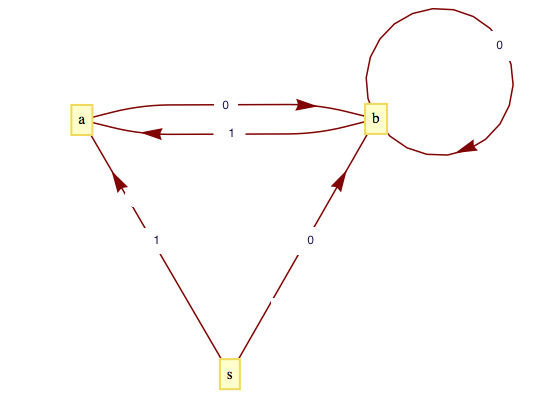
\includegraphics[width=1\linewidth]{images/fig-directed-graph-ex1.png}
\caption{An undirected graph\label{fig-directed-graph-ex1}}
\end{figure}
\end{example}
\par
In certain cases there may be a need for more than one edge between two vertices, and we need to expand the class of directed graphs.%
\begin{definition}[Multigraph.]\label{def-multigraph}
\index{Multigraph}\index{Multigraph}
 A multigraph is a set of vertices \(V\) with a set of edges that can contain more than one edge between the vertices.%
\end{definition}
\par
One important point to keep in mind is that if we identify a graph as being a multigraph, it isn't necessary that there are two or more edges between some of the vertices.  It is only just \emph{allowed}. In other words, every simple graph is a multigraph. This is analogous to how a rectangle is a more general geometric figure than a square, but a square is still considered a rectangle.%
\begin{example}[A Multigraph]\label{ex-multigraph-9-1}
 A Multigraph. A common occurrence of a multigraph is a road map. The cities and towns on the map can be thought of as vertices, while the roads are the edges. It is not uncommon to have more than one road connecting two cities. In order to give clear travel directions, we name or number roads so that there is no ambiguity. We use the same method to describe the edges of the multigraph in \hyperref[fig-multigraph-ex1]{Figure~\ref{fig-multigraph-ex1}}. There is no question
what \(\textrm{e3}\) is; however, referring to the edge \((2, 3)\) would be ambiguous.
%
\leavevmode%
\begin{figure}
\centering
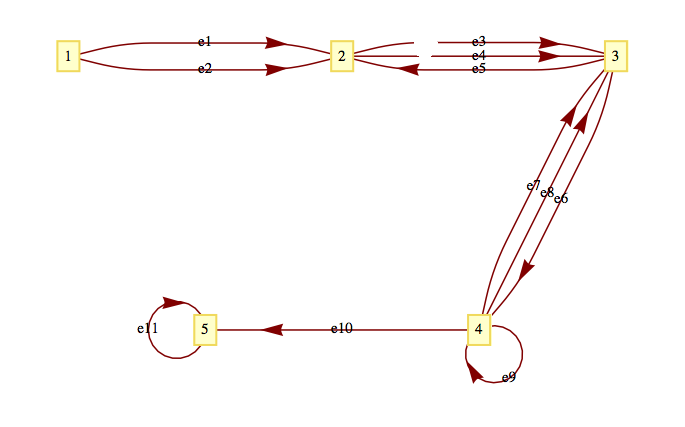
\includegraphics[width=1\linewidth]{images/fig-multigraph-ex1.png}
\caption{An undirected graph\label{fig-multigraph-ex1}}
\end{figure}
\end{example}
\par
There are cases where the order of the vertices is not significant and so we use a different mathematical model for this situation:%
\begin{definition}[Undirected Graph]\label{def-undirected-graph}
\index{Undirected Graph. }\label{notation-1}
An undirected graph consists of a set \(V\), called a vertex set, and a set \(E\) of two-element subsets of \(V\), called the edge set. The two-element subsets are drawn as lines connecting the vertices.%
\end{definition}
\begin{example}[An Undirected Graph]\label{ex-undirected-1}
A network of computers can be described easily using a graph.  \hyperref[fig-undirected-1]{Figure~\ref{fig-undirected-1}} describes a network of five
computers, \(a\), \(b\), \(c\), \(d\), and \(e\). An edge between any two vertices indicates that direct two-way communication
is possible between the two computers. Note that the edges of this graph are not directed. This is due to the fact that the relation that is being
displayed is symmetric (i.e., if \(X\) can communicate with \(Y\), then \(Y\) can communicate with \(X\)). Although directed
edges could be used here, it would simply clutter the graph.%
% group protects changes to lengths, releases boxes (?)
{% begin: group for a single side-by-side
% set panel max height to practical minimum, created in preamble
\setlength{\panelmax}{0pt}
\newsavebox{\panelboxCimage}
\savebox{\panelboxCimage}{
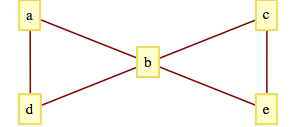
\includegraphics[width=0.5\linewidth]{images/fig-undirected-1.png}
}
\newlength{\phCimage}\setlength{\phCimage}{\ht\panelboxCimage+\dp\panelboxCimage}
\settototalheight{\phCimage}{\usebox{\panelboxCimage}}
\setlength{\panelmax}{\maxof{\panelmax}{\phCimage}}
\newsavebox{\panelboxDimage}
\savebox{\panelboxDimage}{
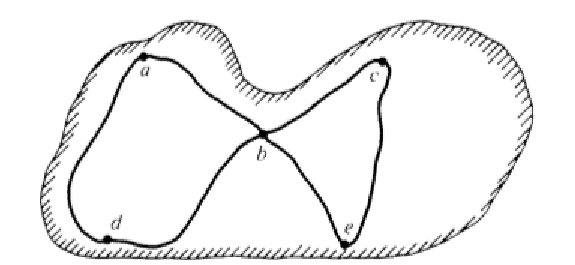
\includegraphics[width=0.5\linewidth]{images/fig-undirected-2.png}
}
\newlength{\phDimage}\setlength{\phDimage}{\ht\panelboxDimage+\dp\panelboxDimage}
\settototalheight{\phDimage}{\usebox{\panelboxDimage}}
\setlength{\panelmax}{\maxof{\panelmax}{\phDimage}}
\leavevmode%
% begin: side-by-side as figure/tabular
% \tabcolsep change local to group
\setlength{\tabcolsep}{0\textwidth}
% @{} suppress \tabcolsep at extremes, so margins behave as intended
\begin{figure}
\begin{tabular}{@{}*{2}{c}@{}}
\begin{minipage}[c][\panelmax][t]{0.5\textwidth}\usebox{\panelboxCimage}\end{minipage}&
\begin{minipage}[c][\panelmax][t]{0.5\textwidth}\usebox{\panelboxDimage}\end{minipage}\tabularnewline
\parbox[t]{0.5\textwidth}{\subcaption{\label{fig-undirected-1}}
}&
\parbox[t]{0.5\textwidth}{\subcaption{\label{fig-undirected-2}}
}\end{tabular}
\caption{Two embeddings of the same undirected graph\label{fig-sidebyside-9-1}}
\end{figure}
% end: side-by-side as tabular/figure
}% end: group for a single side-by-side
\par
This undirected graph, in set terms,  is \(V = \{a, b, c, d, e\}\) and \(E = \{\{a, b,\}, \{a, d\}, \{b, c\}, \{b, d\}, \{c, e\}, \{b, e\}\}\).%
\par
There are several other situations for which this graph can serve as a model. One of them is to interpret the vertices as cities and the edges as roads, an abstraction of a map such as the one in \hyperref[fig-undirected-2]{Figure~\ref{fig-undirected-2}} . Another interpretation is as an abstraction of the floor plan of a house.  See \hyperlink{exercise-house-9-1}{Exercise~1.1.1.11}. Vertex \(a\) represents the outside of the house; all others represent rooms. Two vertices are connected if there is a door between
them. %
\end{example}
\begin{definition}[Complete Undirected Graph.]\label{def-complete-undirected-graph}
\index{Complete Undirected Graph.}\label{notation-2}
A complete undirected graph of \(n\) vertices is an undirected graph with the property that each pair of distinct vertices are connected to one another. Such a graph is usually denoted by \(K_n\).%
\end{definition}
\begin{example}[A Labeled Graph]\label{ex-labeled-graph-9-1}
 A flowchart is a common example of a simple graph that requires labels for its vertices and some of its edges. \hyperref[fig-labeled-graph-9-1]{Figure~\ref{fig-labeled-graph-9-1}}
is one such example that illustrates how many problems are solved. 
%
\leavevmode%
\begin{figure}
\centering
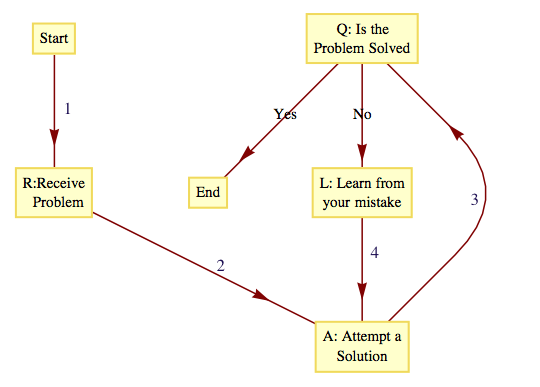
\includegraphics[width=1\linewidth]{images/fig-labeled-graph-9-1.png}
\caption{A flow chart - an example of a labeled graph\label{fig-labeled-graph-9-1}}
\end{figure}
\par
At the start of the problem-solving process, we are at the vertex labeled ``Start'' and at the end (if we are lucky enough to have solved the
problem) we will be at the vertex labeled ``End.'' The sequence of vertices that we pass through as we move from ``Start'' to ``End''
is called a path. The ``Start'' vertex is called the initial vertex of the path, while the ``End'' is called the final, or terminal, vertex.
Suppose that the problem is solved after two attempts; then the path that was taken is \(\text{Start}, R, A, Q, L, A, Q, \text{End}\). An alternate
path description would be to list the edges that were used: \(1, 2, 3, \text{No}, 4, 3, \text{Yes}\). This second method of describing a path has
the advantage of being applicable for multigraphs. On the graph in Figure 9.1.5, the vertex list \(1,2,3,4,3\) does not clearly describe a path between
1 and 3, but \(e_1,e_4, e_6, e_7\) is unambiguous.%
\end{example}
\begin{note}[>A Summary of Path Notation and Terminology]\label{note-2}
If \(x\) and \(y\) are two vertices of a graph, then a \terminology{path} between \(x\) and \(y\) describes a motion from \(x\) and
\(y\) along edges of the graph. Vertex \(x\) is called the initial vertex of the path and \(y\) is called the terminal vertex.
A path between \(x\) and \(y\) can always be described by its  edge list, the list of edges that were used: \(\left(e_1, e_2,
\ldots , e_n\right)\), where : (1) the initial vertex of \(e_1\) is \(x\); (2) the terminal vertex of \(e_i\) is the initial vertex of \(e_{i+1}\), \(i = 1, 2, \ldots , n - 1\); and (3) the terminal vertex of \(e_n\) is \(y\). The number of edges in the edge list is the \terminology{path length}. A path on a simple graph can also be described by a vertex list. A path of length \(n\) will have a list of \(n + 1\) vertices
\(v_0=x\), \(v_1\), \(v_2,\ldots ,v_n=y\), where, for \(k = 0,1,2,\ldots , n-1\), \(\left(v_k,v_{k+1}\right)\) is an edge on the graph. A \terminology{
circuit} is a path that terminates at its initial vertex.%
\par
Suppose that a path between two vertices has an edge list \((e_1, e_2 , . . . ,e_n)\). A \terminology{subpath} of this graph is any portion of the path described by one or more consecutive edges in the edge list. For example, \((3, \textrm{No}, 4)\) is a subpath of \((1,2,3, \textrm{No}, 4, 3, \text{Yes})\).  Any path is its own subpath; however, we call it an improper subpath of itself. All other nonempty subpaths are called proper subpaths.%
\par
A path or circuit is  simple if it contains no proper subpath that is a circuit. This is the same as saying that a path or circuit is simple
if it does not visit any vertex more than once except for the common initial and terminal vertex in the circuit. In the problem-solving method described in \hyperref[fig-labeled-graph-9-1]{Figure~\ref{fig-labeled-graph-9-1}}, the path that you take is simple only if you reach a solution on the first try.%
\end{note}
\begin{example}[An Organizational Graph]\label{organizational-graph}
The leadership structure of a corporation is often represented with a graph as in \hyperref[fig-organization-9-1]{Figure~\ref{fig-organization-9-1}} %
\leavevmode%
\begin{figure}
\centering
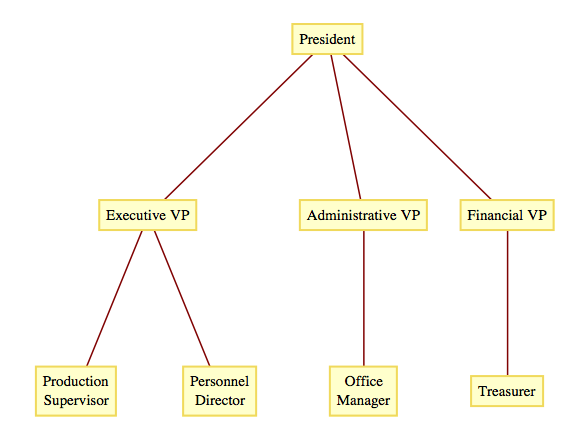
\includegraphics[width=1\linewidth]{images/fig-organization-9-1.png}
\caption{An Organization Graph
                \label{fig-organization-9-1}}
\end{figure}
\par
The principle behind such a structure is that everyone but the president has a single immediate supervisor. Any action that anyone takes can reach
the president only through a unique ``chain of command.'' This chain-of-command property is characteristic of a special type of graph called
a  tree. Note that the edges of this graph are not directed, but, as in a Hasse diagram, the relation between two connecting vertices is
clear: the top vertex is the supervisor of the lower vertex.%
\par
The process of structured (or top-down) problem solving results in a graph that is similar to this tree. Starting with the top of the tree, which
would represent the whole problem, the problem is divided into a sequence of separate subproblems. Each subproblem is divided further into smaller
sub-problems in the same way until the solutions of the lowest problems are easy enough to recognize.
%
\end{example}
\par
From the examples we've see so far, we can see that although a graph can be defined, in short, as a collection of vertices and edges, an integral part of most graphs is the labeling of the vertices and edges that allows us to interpret the graph as a model for some situation. We continue with a few more examples to illustrate this point.%
\begin{example}[A Graph as a Model for a Set of Strings]\label{ex-string-model-9-1}
Suppose that you would like to mechanically describe the set of strings of 0's and
1's having no consecutive 1's. One way to visualize a string of this kind is with the graph in \hyperref[fig-directed-graph-ex1]{Figure~\ref{fig-directed-graph-ex1}}. Consider any path starting at vertex \(s\). If the label on each graph is considered to be the output to a printer, then the output will have no consecutive 1's. For example, the path that is described by the vertex list \((s,a, b, b, a, b, b, a, b)\) would result in an output of \(10010010\). Conversely, any string with  no consecutive 1's determines a path starting at s.
%
\end{example}
\begin{example}[A Tournament Graph.]\label{ex-tournament-graph-9-1}
Suppose that four teams compete in a round-robin sporting event; that is, each team meets every other team
once, and each game is played until a winner is determined. If the teams are named A, B, C, and D, we can define the relation \(\beta\) on the set
of teams by \(X \beta  Y\) if \(X\) beat \(Y\). For one set of results, the graph of \(\beta\) might look like \hyperref[fig-tournament-graph-9-1]{Figure~\ref{fig-tournament-graph-9-1}}.%
\leavevmode%
\begin{figure}
\centering
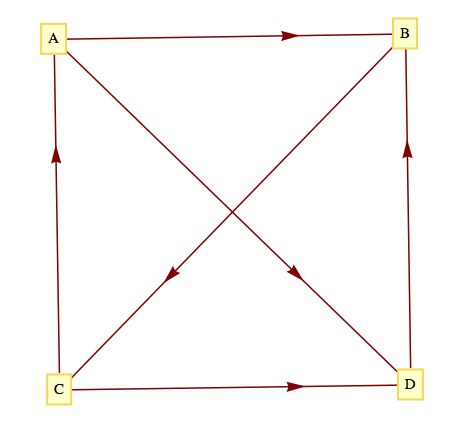
\includegraphics[width=1\linewidth]{images/fig-tournament-graph-9-1.png}
\caption{Round-robin tournament graph with four vertices
                \label{fig-tournament-graph-9-1}}
\end{figure}
\end{example}
\par
There are many types of tournaments and they all can be modeled by different types of graphs.%
\begin{definition}[Tournament Graph]\label{def-tournament-graph}
\index{Tournament Graph}\leavevmode%
\begin{enumerate}[label=\alph*]
\item\hypertarget{li-1}{} A tournament graph is a directed graph with the property that no edge connects a vertex to itself, and between any two vertices there is at most one edge.%
\item\hypertarget{li-2}{}A complete (or round-robin) tournament graph is a tournament graph with the property that between any two distinct vertices there is exactly
one edge%
\item\hypertarget{li-3}{}A single-elimination tournament graph is a tournament graph with the properties that: (i) one vertex (the champion) has no edge terminating
at it and at least one edge initiating from it; (ii) every other vertex is the terminal vertex of exactly one edge; and (iii) there is a path from
the champion vertex to every other vertex.%
\end{enumerate}
%
\end{definition}
\begin{example}[Graph of a Single Elimination Tourament]\label{ex-single-elimination-9-1}
 The major league baseball championship is decided with a single-elimination tournament, where each ``game'' is actually
a series of games. Until 1995, the two divisional champions in the American League (East and West) compete in a series of games. The loser is eliminated and the winner competes against the winner of the National League series (which is decided as in the American League). The tournament graph of the
1983 championship is in \hyperref[fig-mlb-1983-9-1]{\ref{fig-mlb-1983-9-1}}%
\leavevmode%
\begin{figure}
\centering
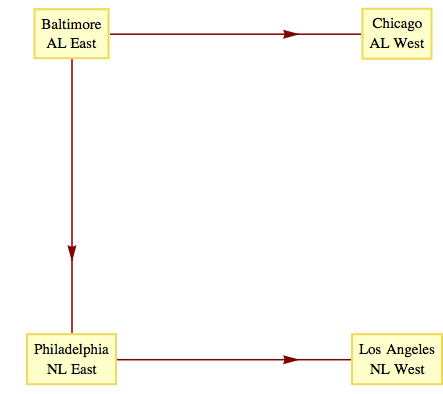
\includegraphics[width=1\linewidth]{images/fig-mlb-1983-9-1.png}
\caption{A single elimination tournament graph
		 \label{fig-mlb-1983-9-1}}
\end{figure}
\end{example}
\par
Next, we establish the relation ``is isomorphic to,'' a form of equality on graphs. The graphs in \hyperref[fig-isomorphic-graphs-9-1]{Figure~\ref{fig-isomorphic-graphs-9-1}} obviously share some similarities, such as the number of vertices and the number of edges. It happens that they are even more similar than just that. If the letters a, b, c, and d in left graph are replaced with the numbers 1,3,4, and 2, respectively, and the vertices are moved around so that they have the same position as the graph on the right, you get the graph on the right.%
\leavevmode%
\begin{figure}
\centering
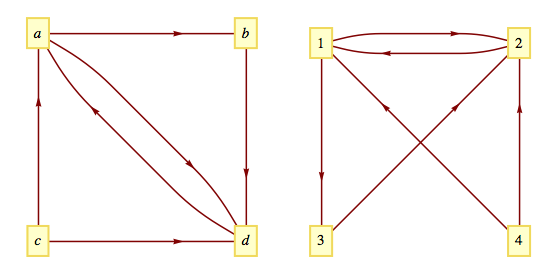
\includegraphics[width=1\linewidth]{images/fig-isomorphic-graphs-9-1.png}
\caption{Isomorphic Graphs
                \label{fig-isomorphic-graphs-9-1}}
\end{figure}
\par
Here is a more precise definition that reflects the fact that the actual positioning (or embedding) of vertices isn't an essential part of a graph.%
\begin{definition}[Isomorphic Graphs]\label{def-isomorphic-graphs.}
\index{Isomorphic Graphs}Two graphs \((V, E)\) and \((V', E')\) are isomorphic if there exists a bijection \(f:V\to V'\) such that \(\left(v_i,v_j\right)\in
E\) if and only if \(\left(f\left(v_i\right),f\left(v_j\right)\right)\in E'\). For multigraphs, we add that the number of edges connecting \(v_i\)
to \(v_j\), must equal the number of edges from \(f\left(v_i\right)\) to \(f\left(v_j\right)\).%
\end{definition}
\par
The most significant local characteristic of a vertex within a graph is its degree.
 Collectively, the degrees can partially characterize a graph.%
\begin{definition}[Degree of a vertex]\label{def-degree-of-a-vertex}
\index{Degree}\label{notation-3}
\leavevmode%
\begin{enumerate}[label=\alph*]
\item\hypertarget{li-4}{} Let v be a vertex of an undirected graph. The degree of v, denoted \textup{ deg}(v), is the number of edges that connect v to the other vertices in the graph.%
\item\hypertarget{li-5}{} If v is a vertex of a directed graph, then the outdegree of v, denoted \textup{ outdeg}(v), is the number of edges of the graph that initiate
at v. The indegree of v, denoted \textup{ indeg}(v). is the number of edges that terminate at v.%
\end{enumerate}
%
\end{definition}
\begin{definition}[Degree Sequence of a Graph]\label{def-degree-sequence}
\index{Degree Sequence of a Graph}The degree sequence of a simple undirected graph is the non-increasing sequence of its vertex degrees.%
\end{definition}
\begin{example}[Some degrees]\label{ex-degrees-9-1}
\leavevmode%
\begin{figure}
\centering
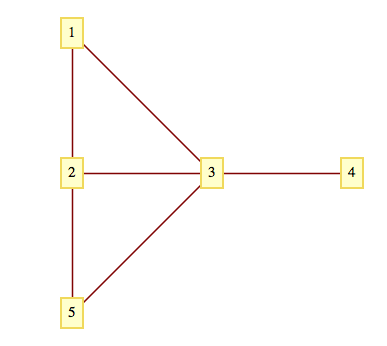
\includegraphics[width=1\linewidth]{images/fig-degrees-example-9-1.png}
\end{figure}
\leavevmode%
\begin{enumerate}[label=\alph*]
\item\hypertarget{li-6}{} The degrees of vertices 1 through 5 in \hyperref[ex-degrees-9-1]{Example~\ref{ex-degrees-9-1}} are 2, 3, 4, 1, and 2, respectively.  The degree sequence of the graph is \((4,3,2,2,1)\)%
\item\hypertarget{li-7}{} In a tournament graph, \(\text{outdeg}(v)\) is the number of wins for \(v\) and \(\text{indeg}(v)\) is the number of losses. In a complete(round-robin) tournament graph with \(n\) vertices, \(\text{outdeg}(v) + \text{indeg}(v) = n - 1\) for each vertex.%
\end{enumerate}
%
\end{example}
\begin{definition}[Graphic Sequences]\label{def-graphic-sequence}
\index{Graphic Sequence}A finite nonincreasing sequence of integers \(d_1,d_2, \ldots , d_n\) is a  graphic if there exists a simple graph with  n vertices
having the sequence as its degree sequence.%
\end{definition}
\par
 For example, \(4,2,1,1,1,1\) is graphic because the degrees of the graph in \hyperref[fig-degree-sequence-example]{Figure~\ref{fig-degree-sequence-example}}
 match these numbers.%
\leavevmode%
\begin{figure}
\centering
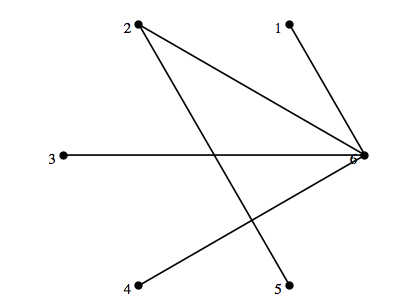
\includegraphics[width=1\linewidth]{images/fig-degree-sequence-example.png}
\caption{Note: There is no connection between the vertex name/number and its degree.
                \label{fig-degree-sequence-example}}
\end{figure}
\begin{listwrapper}[A Prospectus for the Rest of the Chapter]\label{list-graph-prospectus}
\typeout{************************************************}
\typeout{Introduction  }
\typeout{************************************************}
The question ``Once you have a graph, what do you do with it?'' might come to mind. The following list of common questions and comments about
graphs is a partial list that will give you an overview of the remainder of the chapter.%
\leavevmode%
\begin{enumerate}[label=\arabic*]
\item\hypertarget{li-8}{}How can a graph be represented as a data structure for use on a computer? We will discuss some common Pascal data structures that are
used to represent graphs in Section 9.2.%
\item\hypertarget{li-9}{}Given two vertices in a graph, does there exist a path between them? The existence of a path between any or all pairs
of vertices in a graph will be discussed in Section 9.3. A related question is: How many paths of a certain type or length are there between two
vertices?%
\item\hypertarget{li-10}{} Is there a path (or circuit) that passes through every vertex (or uses every edge) exactly once? Paths of this kind are called traversals.
We will discuss traversals in Section 9.4.%
\item\hypertarget{li-11}{}Suppose that a cost is associated with the use of each vertex and/or edge in a path. What is the ``cheapest'' path, circuit, or traversal
of a given kind? Problems of this kind will be discussed in Section 9.5.%
\item\hypertarget{li-12}{}Given the specifications of a graph, or the graph itself, what is the best way to draw the graph? The desire for neatness alone makes this
a reasonable question, but there are other motivations. Another goal might be to avoid having edges of the graph cross one another. This is discussed in Section 9.6.%
\end{enumerate}
\end{listwrapper}
\typeout{************************************************}
\typeout{Exercises 1.1.1 Exercises for Section 9.1}
\typeout{************************************************}
\subsection[Exercises for Section 9.1]{Exercises for Section 9.1}\label{exercises-9-1}
\hypertarget{exercisegroup-1}{}\typeout{************************************************}
\typeout{Introduction  }
\typeout{************************************************}
A Exercises%
\begin{exercisegroup}
\item[1.]\hypertarget{exercise-1}{} What is the significance of the fact that there is a path connecting vertex \(b\) with every other vertex in \hyperref[fig-undirected-1]{Figure~\ref{fig-undirected-1}}, as it applies to various situations that it models?%
\par\smallskip
\item[2.]\hypertarget{exercise-2}{} Draw a graph similar to \hyperref[fig-directed-graph-ex1]{Figure~\ref{fig-directed-graph-ex1}} that represents the set of strings of 0's and 1's containing no more than two consecutive 1's.%
\par\smallskip
\item[3.]\hypertarget{exercise-3}{} Draw a directed graph that models the set of strings of 0's and 1's where all of the 1's must appear consecutively. %
\par\smallskip
\item[4.]\hypertarget{exercise-4}{} In the NCAA final-four basketball tournament, the East champion plays the West champion, and the champions from the Mideast and Midwest play. The winners of the two games play for the national championship. Draw the eight different single-elimination tournament graphs that could occur.%
\par\smallskip
\item[5.]\hypertarget{exercise-5}{} What is the maximum number of edges in a simple undirected graph with eight vertices?%
\par\smallskip
\item[6.]\hypertarget{exercise-6}{} Which of the graphs in \hyperref[fig-exercise-9-1-6]{Figure~\ref{fig-exercise-9-1-6}} are isomorphic? What is the correspondence between their vertices?%
\leavevmode%
\begin{figure}
\centering
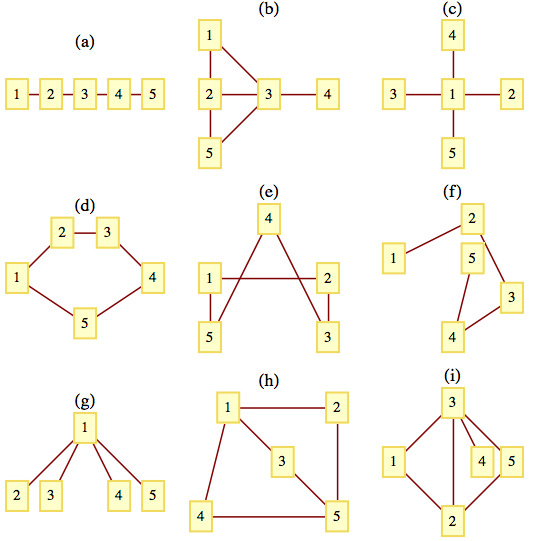
\includegraphics[width=1\linewidth]{images/fig-exercise-9-1-6.png}
\caption{Which graphs are isomorphic to one another?
                \label{fig-exercise-9-1-6}}
\end{figure}
\par\smallskip
\item[7.]\hypertarget{exercise-7}{}\leavevmode%
\begin{enumerate}[label=\alph*]
\item\hypertarget{li-13}{}How many edges does a complete tournament graph with \(n\) vertices have?%
\item\hypertarget{li-14}{}How many edges does a single-elimination tournament graph with n vertices have?%
\end{enumerate}
%
\par\smallskip
\item[8.]\hypertarget{exercise-8}{}Draw complete undirected graphs with 1, 2, 3, 4, and 5 vertices. How many edges does a \(K_n\), a complete undirected graph with \(n\) vertices, have?%
\par\smallskip
\item[9.]\hypertarget{exercise-9}{} Determine whether the following sequences are graphic. Explain your logic.%
\par
\leavevmode%
\begin{enumerate}[label=\alph*]
\item\hypertarget{li-15}{}  \((6, 5, 4, 3, 2, 1, 0)\)%
\item\hypertarget{li-16}{} \((2,2,2,2,2,2)\)%
\item\hypertarget{li-17}{} \((3,2,2,2,2,2)\)%
\item\hypertarget{li-18}{} \((5,3,3,3,3,3)\)%
\item\hypertarget{li-19}{} \((1,1,1,1,1,1)\)%
\item\hypertarget{li-20}{} \((5,5,4,3,2,1)\)%
\end{enumerate}
%
\par\smallskip
\item[10.]\hypertarget{exercise-10}{}\leavevmode%
\begin{enumerate}[label=\alph*]
\item\hypertarget{li-21}{}Based on observations you might have made in exercise 9, describe as many characteristics as you can about graphic sequences of length
\(n\).%
\item\hypertarget{li-22}{} Consider the two graphs in \hyperref[fig-same-ds-9-1]{Figure~\ref{fig-same-ds-9-1}}. Notice that they have the same degree sequences, \((2,2,2,2,2,2)\).  Explain why the two graphs are not isomorphic.%
\end{enumerate}
%
\leavevmode%
\begin{figure}
\centering
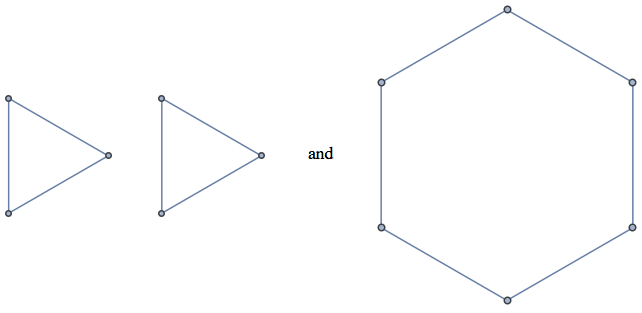
\includegraphics[width=1\linewidth]{images/fig-same-ds-9-1.png}
\caption{Two Graphs with the same degree sequences
                \label{fig-same-ds-9-1}}
\end{figure}
\par\smallskip
\item[11.]\hypertarget{exercise-house-9-1}{}Draw a plan for the rooms of a house so that \hyperref[fig-undirected-1]{Figure~\ref{fig-undirected-1}} models connectedness of the rooms.  That is, \((a,b)\) is an edge if and only if a door connects rooms \(a\) and \(b\). %
\par\smallskip
\end{exercisegroup}
\par\smallskip\noindent
\typeout{************************************************}
\typeout{Section 1.2 Data Structures and Computer Generation of Graphs}
\typeout{************************************************}
\section[Data Structures and Computer Generation of Graphs]{Data Structures and Computer Generation of Graphs}\label{s-data-structures-for-graphs}
\index{Graph!Data Structures}\typeout{************************************************}
\typeout{Introduction  }
\typeout{************************************************}
In this section, we will describe data structures that are commonly used to represent graphs. In addition we will introduce the basic syntax for
graphs in Sage.%
\typeout{************************************************}
\typeout{Subsection 1.2.1 Basic Data Stuctures}
\typeout{************************************************}
\subsection[Basic Data Stuctures]{Basic Data Stuctures}\label{ss-graph-data-structures}
\begin{listwrapper}[Data Structures for Graphs]\label{list-2}
\typeout{************************************************}
\typeout{Introduction  }
\typeout{************************************************}
Assume that we have a graph with \(n\) vertices that can be indexed by the integers \(1, 2, \dots, n\).  Here are three different data structures that can be employed to represent graphs.%
\leavevmode%
\begin{enumerate}
\item\hypertarget{li-23}{}Adjacency Matrix:  As we saw in Chapter 6, the information about edges in a graph can be summarized with an adjacency
matrix, \(G\), where \(G_{\text{ij}}=1\) if and only if vertex \(i\) is connected to vertex \(j\) in the graph.  Note
that this is the same as the adjacency matrix for a relation, with the exception.%
\item\hypertarget{li-24}{}Edge Dictionary:  For each vertex in our graph, we maintain a list of edges that
initiate at that vertex. If \(G\) represents the graph's edge information, then we denote by \(G_i\) the list of vertices that are terminal vertices  of edges initiating at vertex \(i\). The exact syntax that would be used can vary.  We will use the Python syntax that is adopted be used in Sage.%
\item\hypertarget{li-25}{}Edge List:  Note that in creating either of the first two data structures, we would presume that a list of
edges for the graph exists. A simple way to represent the edges is to maintain this list of ordered pairs, or two element sets, depending on whether the graph is intended to be directed or undirected.  We will not work with this data stucture here, other than in the first example.%
\end{enumerate}
\end{listwrapper}
\begin{example}[A Very Small Example]\label{ex-data-structure-sample}
We consider the representation of the following graph:%
\leavevmode%
\begin{figure}
\centering
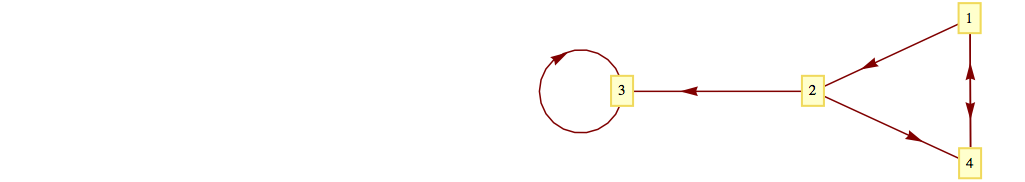
\includegraphics[width=1\linewidth]{images/fig-example-9-2-1.png}
\end{figure}
\par
The adjacency matrix that represents the graph would be 
\(\quad \quad\)\(G=\left(
\begin{array}{cccc}
 0 & 1 & 0 & 1 \\
 0 & 0 & 1 & 1 \\
 0 & 0 & 1 & 0 \\
 1 & 0 & 0 & 0 \\
\end{array}
\right)\).%
\par
The same graph would be represented with the edge dictionary 
\lstinline?{1:[2,4],2:[3,4],3:[3],4:[1]}?.  Notice the general form of each item in the dictionary: \lstinline?vertex:[list of vertices]?.%
\par
Finally, the list of edges \(\{(1,2),(1,4),(2,3),(2,4),(3,3),(4,1)\}\) also describes the same graph.%
\end{example}
A natural question to ask is: Which data structure should be used in a given situation? For small graphs, it really doesn't make much difference.  For larger matrices the edge count would be a consideration. If \(n\) is large and the
number of edges is relatively small, it might use less memory to maintain an edge dictionary or  list of edges instead of building an \(n \times  n\) matrix. Some software for working with graphs will make the decision for you.%
\begin{example}[NCAA Basketball]\label{ex-ncaa-bb}
Consider an directed graph represented by the Division I NCAA college basketball teams in the United States for a given year. There are approximately 350 teams in Division 1. Suppose we constructed the graph with an edge from team A to team B if A beat B at least once in the season; and we label the edge with the number of wins.  Since the average team plays around 30 games in a season, most of which will be against other Division I teams, we could expect around \(\frac{30 \cdot 350}{2}=5,250\) edges in the graph. This would be somewhat reduced by games with lower division teams and cases where two or more wins over the same team produces one edge. Since 5,250 is much smaller than \(350^2=122,500\) entries in an adjacency matrix.  Clearly, an edge dictionary or edge list would be more compact than an adjacency matrix.  Even if we were use software to create an adjacency matrix, many programs will identify the fact that a matrix such as the one in this example would be "sparse" and would leave data in list form and use sparse array methods to work with it.%
\end{example}
\typeout{************************************************}
\typeout{Subsection 1.2.2 Sage Graphs}
\typeout{************************************************}
\subsection[Sage Graphs]{Sage Graphs}\label{sss-sage-graphs}
\index{Sage Note!Graphs}The most common way to define a graph in Sage is to use an edge dictionary.  Here is how the graph in \hyperref[ex-data-structure-sample]{Example~\ref{ex-data-structure-sample}} is generated and then displayed.  Notice that  we simply wrap the function \lstinline?DiGraph()? around the same dictionary expression we identified earlier.%
\begin{lstlisting}[style=sageinput]
G1 = DiGraph( {1 : [4, 2], 2 : [3, 4], 3 : [3], 4 : [1]})
G1.show()
\end{lstlisting}
\par

You can get the adjacency matrix of a graph with the \lstinline?adjacency_matrix? method.
%
\begin{lstlisting}[style=sageinput]
G1.adjacency_matrix()
\end{lstlisting}
\begin{lstlisting}[style=sageoutput]
[0 1 0 1]
[0 0 1 1]
[0 0 1 0]
[1 0 0 0]
\end{lstlisting}
\par
You can also define a graph based on its adjacency matrix.%
\begin{lstlisting}[style=sageinput]
M = Matrix([[0,1,0,0,0],[0,0,1,0,0],[0,0,0,1,0],
			[0,0,0,0,1],[1,0,0,0,0]])
DiGraph(M).show()
\end{lstlisting}
\begin{lstlisting}[style=sageoutput]
[0 1 0 1]
[0 0 1 1]
[0 0 1 0]
[1 0 0 0]
\end{lstlisting}
\par
The edge list of any directed graph an be easily retrieved.  If you replace \lstinline?edges? with \lstinline?edge_iterator?, you can iterate through the edge list.  The third coordinate of the items in the edge is the label of the edge, which is None in this case.%
\begin{lstlisting}[style=sageinput]
DiGraph(M).edges()
\end{lstlisting}
\begin{lstlisting}[style=sageoutput]
[(0, 1, None), (1, 2, None), (2, 3, None), (3, 4, None), (4, 0, None)]
\end{lstlisting}
\par
Replacing the wrapper \lstinline?DiGraph()? with \lstinline?Graph()? creates an undirected graph.%
\begin{lstlisting}[style=sageinput]
G2 = Graph( {1 : [4, 2], 2 : [3, 4], 3 : [3], 4 : [1]})
G2.show()
\end{lstlisting}
\par
There are many special graphs and graph families that are available in Sage through the \lstinline?graphs? module.  They are referenced with the prefix \lstinline?graphs.? followed by the name and zero or more paramenters inside parentheses.  Here are a couple of them, first a complete graph with five vertices.%
\begin{lstlisting}[style=sageinput]
graphs.CompleteGraph(5).show()
\end{lstlisting}
\par
Here is a wheel graph, named for an obvious pattern of vertices and edges.  We assign a name to it first and then show the graph without labeling the vertices.%
\begin{lstlisting}[style=sageinput]
w=graphs.WheelGraph(20)
w.show(vertex_labels=false)
\end{lstlisting}
\par
There are dozens of graph methods, one of which determines the degree sequence of a graph.  In this case, it's the wheel graph above %
\begin{lstlisting}[style=sageinput]
w.degree_sequence()
\end{lstlisting}
\begin{lstlisting}[style=sageoutput]
[19, 3, 3, 3, 3, 3, 3, 3, 3, 3, 3, 3, 3, 3, 3, 3, 3, 3, 3, 3]
\end{lstlisting}
\par
The degree sequence method is defined within the graphs module, but the prefix \lstinline?graphs.? is not needed because the value of \lstinline?w? inherits the graphs methods.%
\typeout{************************************************}
\typeout{Exercises 1.2.3 Exercises for Section 9.2}
\typeout{************************************************}
\subsection[Exercises for Section 9.2]{Exercises for Section 9.2}\label{exercises-9-2}
\hypertarget{exercisegroup-2}{}\typeout{************************************************}
\typeout{Introduction  }
\typeout{************************************************}
A Exercises%
\begin{exercisegroup}
\item[1.]\hypertarget{exercise-12}{}Estimate the number of vertices and edges in each of the following graphs. Would the graph be considered sparse, so that an adjacency matrix would be inefficient?%
\par
\leavevmode%
\begin{enumerate}[label=\alph*]
\item\hypertarget{li-26}{} Vertices: Cities of the world that are served by at least one airline. 
  Edges: Pairs of cities that are connected by a regular direct flight.%
\item\hypertarget{li-27}{} Vertices: ASCII characters. 
 Edges: connect characters that differ in their binary code by exactly two bits.%
\item\hypertarget{li-28}{} Vertices: All English words. 
 Edges: An edge connects word x to word y if x is a prefix of y.%
\end{enumerate}
%
\par\smallskip
\par\smallskip
\noindent\textbf{Answer.}\hypertarget{answer-1}{}\quad
\leavevmode%
\begin{enumerate}[label=\alph*]
\item\hypertarget{li-29}{}  A rough estimate of the number of vertices in the ``world airline graph'' would be the number of cities with population greater than or equal to 100,000. This is estimated to be around 4,100. There are many smaller cities that have airports, but some of the metropolitan areas with clusters of large cities are served by only a few airports.  4,000-5,000 is probably a good guess.   As for edges, that's a bit more difficult to estimate.  It's certainly not  a complete graph.  Looking at some medium sized airports such as Manchester, NH, the average number of cities that you can go to directly is in the 50-100 range.   So a very
rough estimate would be   \(\frac{75 \cdot  4500}{2}=168,750\). This is far less than \(4,500^2\), so an edge list or dictionary of some kind would be more efficient. %
\item\hypertarget{li-30}{} The number of ASCII characters is 128.  Each character would be connected to \(\binom{8}{2}=28\) others and so there are \(\frac{128 \dot 28}{2}=3,584\)  edges.  Comparing this to the \(128^2=16,384\), an array is probably the best choice.
%
\item\hypertarget{li-31}{} The Oxford English Dictionary as approximately a half-million words, although many are obsolete.   The number of edges is probably of the same order of magnitude as the number of words, so an edge list or dictionary is probably the best choice.%
\end{enumerate}
%
\item[2.]\hypertarget{exercise-13}{} Each edge of a graph is colored with one of the four colors red, blue, yellow, or green. How could you represent the edges in this graph using
a variation of the adjacency matrix structure?%
\par\smallskip
\item[3.]\hypertarget{exercise-14}{}Directed graphs \(G_1, \dots, G_6\) , each with vertex set \(\{1,2,3,4,5\}\) are represented by the matrices below. Which graphs are isomorphic to one another?%
\par
 \(G_1: \left(
\begin{array}{ccccc}
 0 & 1 & 0 & 0 & 0 \\
 0 & 0 & 1 & 0 & 0 \\
 0 & 0 & 0 & 1 & 0 \\
 0 & 0 & 0 & 0 & 1 \\
 1 & 0 & 0 & 0 & 0 \\
\end{array}
\right)\)\(\quad \quad\)\(G_2: \left(
\begin{array}{ccccc}
 0 & 0 & 0 & 0 & 0 \\
 0 & 0 & 1 & 0 & 0 \\
 0 & 0 & 0 & 0 & 0 \\
 1 & 1 & 1 & 0 & 1 \\
 0 & 0 & 0 & 0 & 0 \\
\end{array}
\right)\)\(\quad \quad\)\(G_3: \left(
\begin{array}{ccccc}
 0 & 0 & 0 & 0 & 0 \\
 1 & 0 & 0 & 0 & 1 \\
 0 & 1 & 0 & 0 & 0 \\
 0 & 0 & 1 & 0 & 0 \\
 0 & 0 & 1 & 0 & 0 \\
\end{array}
\right)\)

 \(G_4: \left(
\begin{array}{ccccc}
 0 & 1 & 1 & 1 & 1 \\
 0 & 0 & 0 & 0 & 0 \\
 0 & 0 & 0 & 0 & 0 \\
 0 & 0 & 1 & 0 & 0 \\
 0 & 0 & 0 & 0 & 0 \\
\end{array}
\right)\)\(\quad \quad\)\(\quad G_5: \left(
\begin{array}{ccccc}
 0 & 0 & 0 & 0 & 1 \\
 0 & 0 & 0 & 0 & 0 \\
 0 & 1 & 0 & 1 & 0 \\
 0 & 0 & 0 & 0 & 1 \\
 0 & 0 & 1 & 0 & 0 \\
\end{array}
\right)\)\(\quad \quad\)\(G_6: \left(
\begin{array}{ccccc}
 0 & 0 & 0 & 1 & 0 \\
 0 & 0 & 0 & 0 & 0 \\
 1 & 1 & 0 & 0 & 0 \\
 0 & 0 & 1 & 0 & 0 \\
 0 & 0 & 0 & 1 & 0 \\
\end{array}
\right)\)%
\par\smallskip
\par\smallskip
\noindent\textbf{Answer.}\hypertarget{answer-2}{}\quad
 Each graph is isomorphic to itself. In addition, \(G_2 \text{and} G_4\) are isomorphic; and \(G_3,G_5, \text{and and} G_6\) are isomorphic to one another.%
\item[4.]\hypertarget{exercise-15}{} The following Sage command verifies that the wheel graph with four vertices is isomorphic to the complete graph with four vertices. %
\begin{lstlisting}[style=sageinput]
graphs.WheelGraph(4).is_isomorphic(graphs.CompleteGraph(4))
\end{lstlisting}
\begin{lstlisting}[style=sageoutput]
True
\end{lstlisting}
\par
A list of all graphs in this the \lstinline?graphs? database is available via tab
   completion. Type "graphs." and then hit the tab key to see which
   graphs are available.  This can be done using the Sage application or SageMathCloud, but not sage cells.  Find some other pairs of isomorphic graphs in the database.%
\par\smallskip
\end{exercisegroup}
\par\smallskip\noindent
\typeout{************************************************}
\typeout{Section 1.3 Connectivity}
\typeout{************************************************}
\section[Connectivity]{Connectivity}\label{s-Connectivity}
\index{Connectivity in Graphs}\typeout{************************************************}
\typeout{Introduction  }
\typeout{************************************************}
This section is devoted to a question that, when posed in relation to the graphs that we have examined, seems trivial. That question is: Given two
vertices, \(s\) and \(t\), of a graph, is there a path from \(s\) to  t?  If \(s = t\), this question is interpreted
as asking whether there is a circuit of positive length starting at \(s\). Of course, for the graphs we have seen up to now, this question
can be answered after a brief examination.%
\typeout{************************************************}
\typeout{Subsection 1.3.1 Preliminaries}
\typeout{************************************************}
\subsection[Preliminaries]{Preliminaries}\label{ss-connectivity-prelim}
There are two situations under which a question of this kind is nontrivial. One is where the graph is very large and an ``examination'' of the
graph could take a considerable amount of time. Anyone who has tried to solve a maze may have run into a similar problem. The second interesting
situation is when we want to pose the question to a machine. If only the information on the edges between the vertices is part of the data structure
for the graph, how can you put that information together to determine whether two vertices can be connected by a path?%
\begin{note}[Connectivity Terminology]\label{note-3}
 Let \(v\) and \(w\) be vertices of a directed graph. Vertex \(v\) is  connected to vertex
\(w\) if there is a path from \(v\) to \(w\). Two vertices are  strongly connected if they are connected in both directions
to one another. A  graph is connected if, for each pair of distinct vertices, \(v\) and \(w\), \(v\) is connected to \(w\)  or \(w\) is connected to \(v\). A  graph is strongly connected if every pair of its vertices is strongly connected. For an
undirected graph, in which edges can be used in either direction, the notions of strongly connected and connected are the same.%
\end{note}
\begin{theorem}[Maximal Path Theorem]\label{theorem-9.3.1}
If a graph has \(n\) vertices and vertex \(u\) is connected to vertex \(w\), then there exists a path from \(u\) to \(w\) of length no more than
\(n\).%
\end{theorem}
\begin{proof}\hypertarget{proof-1}{}
(Indirect): Suppose \(u\) is connected to \(w\), but the shortest path from \(u\) to \(w\) has length \(m\), where \(m>n\). A vertex list for a path of length \(m\) will have \(m + 1\) vertices. This path can be represented as \(\left(v_0,v_1,\ldots, v_m\right)\), where \(v_0=u\) and \(v_m= w\). Note that since there are only \(n\) vertices in the graph and m vertices are listed in the path after \(v_0\), we can apply the pigeonhole principle and be assured that there must be some duplication in the last \(m\) vertices of the vertex list, which represents a circuit in the path. This means that our path of minimum length can be reduced, which is a contradiction.%
\end{proof}
\begin{listwrapper}[Basic Questions]\label{list-3}
\leavevmode%
\begin{enumerate}
\item\hypertarget{li-32}{}Given a graph and two vertices in the graph, is there a path from the first vertex to the second?%
\item\hypertarget{li-33}{}If the answer to Question 1 is ``yes'' then what is the path?%
\end{enumerate}
\end{listwrapper}
\typeout{************************************************}
\typeout{Subsection 1.3.2 Adjacency Matrix Method}
\typeout{************************************************}
\subsection[Adjacency Matrix Method]{Adjacency Matrix Method}\label{ss-adjacency-matrix-method}
\index{Adjacency Matrix Method}\begin{algorithm}[Adjacency Matrix Method]\label{algorithm-1}
Suppose that the information about edges in a graph is stored in an adjacency matrix, \(G\). The
relation, \(r\), that \(G\) defines is \(v r w\) if there is an edge connecting \(v\) to \(w\). Recall that the composition
of \(r\) with itself, \(r^2\) , is defined by \(v r^2 w\) if there exists a vertex \(y\) such that \(v r y\) and \(y r w\); that is,
\(v\) is connected to \(w\) by a path of length 2. We could prove by induction that the relation \(r^k\) , \(k\geq 1\), is defined by
\(v r^k w\) if and only if there is a path of length \(k\) from \(v\) to \(w\). Since the transitive closure, \(r^+\) , is the
union of \(r\), \(r^2\) \(,r^3,\ldots\), we can answer our connectivity question by determining the transitive closure of \(r\), which
can be done most easily by keeping our relation in matrix form. \hyperref[theorem-9.3.1]{Theorem~\ref{theorem-9.3.1}} is significant in our calculations because it tells us that we need
only go as far as \(E^n\) to determine the matrix of the transitive closure. %
\end{algorithm}
The main advantage of the adjacency matrix method is that the transitive closure matrix can answer all questions about the existence of paths between any 
vertices. If \(G^+\)is the matrix of the transitive closure, \(v_i\), is connected to \(v_j\) if \(\left(E^+\right)_{i j }=1\) . A directed
graph is connected if \(\left(E^+\right)_{i j }=1\) or \(\left(E^+\right)_{j i}=1\) for each \(i\neq j\). A directed graph is strongly connected
if its transitive closure matrix has no zeros.%
\par
A disadvantage of the adjacency matrix method is that the transitive closure matrix tells us whether a path exists, but not what the path is.  The next algorithm solve this problem%
\typeout{************************************************}
\typeout{Subsection 1.3.3 Breadth-First Search}
\typeout{************************************************}
\subsection[Breadth-First Search]{Breadth-First Search}\label{ss-breadth-first-search}
\index{Breadth-First Search}We will describe the Breadth-First Search Algorithm first with an example.%
\par
 The football team at Mediocre State University (MSU) has had a bad year, 2 wins and 9 losses. Thirty days after the end of the football season, the university trustees is meeting to decide whether to rehire the head coach; things look bad for him. However, on the day
of the meeting, the coach issues the following press release with results from the past year:%
\begin{listwrapper}[Press Release: MSU complete successful season]\label{list-4}
\typeout{************************************************}
\typeout{Introduction  }
\typeout{************************************************}
The Mediocre State University football team compared favorably with national champion Enourmous State University this season.%
\leavevmode%
\begin{itemize}[label=\textbullet]
\item{}Mediocre State defeated Local A & M.%
\item{}Local A & M defeated City College.%
\item{}City College defeated Corn State U.%
\item{}... (25 results later)%
\item{}Tough Tech defeated Enormous State University (ESU).%
\end{itemize}
\typeout{************************************************}
\typeout{Conclusion  }
\typeout{************************************************}
\bigbreak
...and ESU went on to win the national championship!%
\end{listwrapper}
\par
The trustees were so impressed that they rehired the coach with a raise! How did the coach come up with such a list?%
\par
In reality, such lists exist occasionally and have appeared in newspapers from time to time. Of course they really don't prove anything since each team that defeated MSU in our example above can produce a similar, shorter chain of results. Since college football records are readily available, the coach could have found this list by trial and error. All that he needed to start with was that his team won at least one game. Since ESU lost one game, there was some hope of producing the chain.%
\par
The problem of finding this list is equivalent to finding a path in the tournament graph for last year's football season that initiates at MSU and ends at ESU. Such a graph is far from complete and is likely to be represented using edge lists. To make the coach's problem interesting,
let's imagine that only the winner of any game remembers the result of the game. The coach's problem has now taken on the flavor of a maze. To reach
ESU, he must communicate with the various teams along the path. One way that the coach could have discovered his list in time is by sending the following
messages to the coaches of the two teams that MSU defeated during the season:%
\begin{note}[]\label{note-4}
When this example was first written, we commented that ties should be ignored. Most recent NCAA rules call for a tiebreaker in college football and so ties are no longer an issue. Email was also not common and we described the process in terms of letter, not email messages. Another change is that the coach could also have asked the MSU math department to use Mathematica or Sage to find the path!%
\end{note}
\begin{listwrapper}[The Coach's Letter]\label{list-5}
\typeout{************************************************}
\typeout{Introduction  }
\typeout{************************************************}
Dear Football Coach:%
\par
Please follow these directions exactly.%
\leavevmode%
\begin{enumerate}
\item\hypertarget{li-39}{} If you are the coach at ESU, contact the coach at MSU now and tell him who sent you this message.%
\item\hypertarget{li-40}{} If you are not the coach at ESU and this is the first message of this type that you have received, then:%
\par
%
\begin{itemize}[label=\textbullet]
\item{}Remember from whom you received this message.%
\item{}Forward a copy of this message, signed by you, to each of the coaches whose teams you defeated during the past year. %
\item{}Ignore this message if you have received one like it already.%
\end{itemize}
%
\end{enumerate}
\typeout{************************************************}
\typeout{Conclusion  }
\typeout{************************************************}
\bigbreak
\(\quad \quad \quad \quad \quad \)Signed,%
\par
\(\quad \quad \quad \quad \quad \)Coach of MSU%
\end{listwrapper}
\begin{listwrapper}[
Observations]\label{list-6}
\typeout{************************************************}
\typeout{Introduction  }
\typeout{************************************************}
From the conditions of this message, it should be clear that if everyone cooperates and if coaches participate within a day of receiving
the message:%
\leavevmode%
\begin{enumerate}[label=\arabic*]
\item\hypertarget{li-44}{} If a path of length \(n\) exists from MSU to ESU, then the coach will know about it in \(n\) days.%
\item\hypertarget{li-45}{} By making a series of phone calls, the coach can construct a path that he wants by first calling the coach who defeated ESU (the person who sent ESU's coach that message). This coach will know who sent him a letter, and so on. Therefore, the vertex list of the desired path is constructed in reverse order.%
\item\hypertarget{li-46}{} If a total of \(M\) football games were played, no more than \(M\) messages will be sent out.%
\item\hypertarget{li-47}{} If a day passes without any message being sent out, no path from MSU to ESU exists.%
\item\hypertarget{li-48}{} This method could be extended to construct a list of all teams that a given team can be connected to. Simply imagine a series of letters like the one above sent by each football coach and targeted at every other coach.%
\end{enumerate}
\end{listwrapper}
\par
The general problem of finding a path between two vertices in a graph, if one exists, can be solved exactly as we solved the problem above. The following
algorithm is commonly called a  breadth-first search.%
\begin{algorithm}[Breadth-first Search]\label{alg-breadth-first}
\index{Breadth-first Search}A broadcasting algorithm for finding a path between vertex \(i\) and vertex \(j\) of a graph having \(n\) vertices. The each item \(V_k\) of a list \(V=\left\{V_1, V_2, \ldots , V_n\right\}\), consist of a Boolean field \(V_k.\text{found}\) and an
integer field \(V_k.\text{from}\). The sets \(D_1\), \(D_2\), \dots, called  depth sets, have the property that if \(k\) is in
\(D_r\) , then the shortest path from vertex \(i\) to vertex \(k\) is of length \(r\). In Step 5, a stack is used to put the vertex list for the path from the vertex \(i\) to vertex \(j\) in the proper order.%
\par
\leavevmode%
\begin{enumerate}[label=\arabic*]
\item\hypertarget{li-49}{}Set the value \(V_k.\text{found}\) equal to False, \(k = 1, 2, \dots , n\)%
\item\hypertarget{li-50}{}\(r = 0\)%
\item\hypertarget{li-51}{} \(D_0= \{i\}\)%
\item\hypertarget{li-52}{} while \((\neg V_j.\text{found}\)) and \(\left(D_r\right.\neq \emptyset )\)%
\par
%
\begin{itemize}[label=\textbullet]
\item{}\(D_{r+1}=\emptyset\)%
\item{} for each k in \(D_r\):%
\par
\(\quad\)for each edge (k,t):%
\par
\(\quad \quad \)If \(V_t.\text{found}\) == False: %
\par
\(\quad \quad \quad \)\(V_t.\text{found}=\text{True}\)%
\par
\(\quad \quad \quad \)\(V_t.\text{from} = k\)%
\par
\(\quad \quad \quad \)\(D_{r+1}=D_{r+1}\cup \{t\}\)%
\item{}\(r = r + 1\)%
\end{itemize}
%
\item\hypertarget{li-56}{}if \(V_j.\text{found} = \text{True}\):%
\par
%
\begin{itemize}[label=\textbullet]
\item{}\(S = Empty Stack\)%
\item{}\(k=j\)%
\item{}while \(V_k.\text{from} \neq  i\):%
\par
\(\quad\)Push \(k\) onto \(S\)%
\par
\(\quad\)\(k = V_k.\text{from}\)%
\end{itemize}
%
\end{enumerate}
%
\end{algorithm}
\begin{listwrapper}[Notes on Breadth-first Search]\label{list-7}
\leavevmode%
\begin{itemize}[label=\textbullet]
\item{} This algorithm will produce one path from vertex \(i\) to vertex \(j\), if one exists, and that path will be as short as possible.
If more than one path of this length exists, then the one that is produced depends on the order in which the edges are examined and the order in
which the elements of \(D_r\) are examined in Step 4.%
\item{} The condition \(D_{r }\neq \emptyset\) is analogous to the condition that if no mail is sent in a given stage of the process, in which
case MSU cannot be connected to ESU.%
\item{} This algorithm can be easily revised to find paths to all vertices that can be reached from vertex i. Step 5 would be put off until a specific
path to a vertex is needed since the information in \(V\) contains an efficient list of all paths. The algorithm can also be extended further
to find paths between any two vertices.%
\end{itemize}
\end{listwrapper}
\begin{example}[A simple example]\label{ex-search-example}
 Consider the graph below. The existence of a path from vertex 2 to vertex 3 is not difficult to determine by examination.
After a few seconds, you should be able to find two paths of length four. Algorithm 9.3.1 will produce one of them.%
\leavevmode%
\begin{figure}
\centering
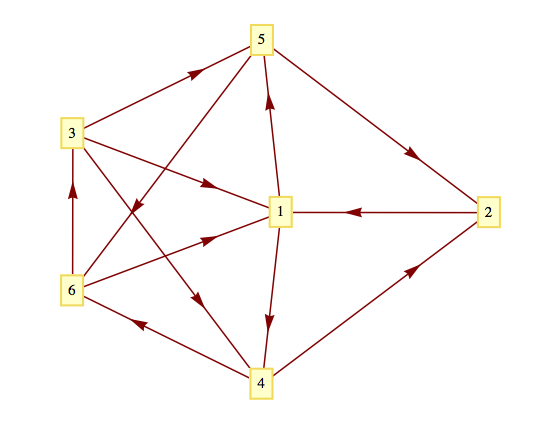
\includegraphics[width=1\linewidth]{images/fig-example-9-3-1.png}
\end{figure}
\par
Suppose that the edges from each vertex are sorted in ascending order by terminal vertex. For example, the edges from vertex 3 would be in the order
\((3, 1), (3, 4), (3, 5)\). In addition, assume that in the body of Step 4 of the algorithm, the elements of \(D_r\) are used in ascending order.  Then at the end of Step 4, the value of V will be

 \[\begin{array}{cccccccc}
 k & 1 & 2 & 3 & 4 & 5 & 6 &   \\
 V_k.\text{found} & T & T & T & T & T & T &   \\
 V_k.\text{from} & 2 & 4 & 6 & 1 & 1 & 4 &   \\
 \text{Depth} \text{set} & 1 & 3 & 4 & 2 & 2 & 3 & \\
\end{array}\]

Therefore, the path \((2, 1, 4, 6, 3)\) is produced by the algorithm. Note that if we wanted a path from 2 to 5, the information in \(V\) produces
the path (2, 1, 5) since \(V_k.\text{from} = 1\) and \(V_1.\text{from} = 2\). A shortest circuit that initiates at vertex 2 is also available
by noting that \(V_2.\text{from}=4\), \(V_4\text{.from = 1}\), and \(V_1.\text{from} = 2\); thus the circuit \((2, 1, 4, 2)\) is the output of the algorithm.
%
\end{example}
\typeout{************************************************}
\typeout{Subsection 1.3.4 Sage Note - Graph Searching}
\typeout{************************************************}
\subsection[Sage Note - Graph Searching]{Sage Note - Graph Searching}\label{ss-sage-note-search}
\index{Sage Note!Search in a Graph}The following sequence of Sage cells illustrates how searching can be done in graphs.%
\par
Generate a random undirected graph with 18 vertices. For each pair of vertices, an edge is included between them with probability 0.2. Since there are \(\binom{18}{2}=153\) potential edges, we expect that there will be approximately \(0.2 \cdot 153 \approx 31\) edges.  The random number generation is seeded first so that the result will always be the same in spite of the random graph function.  Changing or removing that first line will let you experiment with different graphs.%
\begin{lstlisting}[style=sageinput]
set_random_seed(2002)
Gr=graphs.RandomGNP(18,0.2)
Gr.show()
\end{lstlisting}
\par
Count the number of edges. In this case the number is a bit less than expected.%
\begin{lstlisting}[style=sageinput]
len(Gr.edges(labels=False))
\end{lstlisting}
\begin{lstlisting}[style=sageoutput]
27
\end{lstlisting}
\par
Find a shortest path from vertex 0 to vertex 8.%
\begin{lstlisting}[style=sageinput]
Gr.shortest_path(0, 8)
\end{lstlisting}
\begin{lstlisting}[style=sageoutput]
[0, 7, 3, 8]
\end{lstlisting}
\par
Generate a list of vertices that would be reached in a breadth-first search.  The expression \lstinline?Gr.depth_first_search(0)? creates an iterator that is convenient for programming. Wrapping \lstinline?list( )? around the expression shows the order in which the vertices are visited.%
\begin{lstlisting}[style=sageinput]
list(Gr.breadth_first_search(0))
\end{lstlisting}
\begin{lstlisting}[style=sageoutput]
[0, 7, 14, 15, 16, 2, 3, 13, 17, 4, 5, 10, 6, 11, 8, 1, 9, 12]
\end{lstlisting}
\par
Generate a list of vertices that would be reached in a depth-first search.
 In this type of search you travel in one direction away from the starting point until no further new vertices. We will discuss this search later.%
\begin{lstlisting}[style=sageinput]
list(Gr.depth_first_search(0))
\end{lstlisting}
\begin{lstlisting}[style=sageoutput]
[0, 15, 11, 10, 14, 5, 13, 7, 3, 8, 9, 12, 6, 16, 1, 2, 17, 4]
\end{lstlisting}
\typeout{************************************************}
\typeout{Exercises 1.3.5 Exercises for Section 9.3}
\typeout{************************************************}
\subsection[Exercises for Section 9.3]{Exercises for Section 9.3}\label{exercises-9-3}
\hypertarget{exercisegroup-3}{}\typeout{************************************************}
\typeout{Introduction  }
\typeout{************************************************}
A Exercises%
\begin{exercisegroup}
\item[1.]\hypertarget{exercise-16}{} Apply \hyperref[alg-breadth-first]{Algorithm~\ref{alg-breadth-first}} to find a path from 5 to 1 in \hyperref[alg-breadth-first]{Algorithm~\ref{alg-breadth-first}}. What would be the final value of \(V\)? Assume that the terminal vertices
in edge lists and elements of the depth sets are put into ascending order, as we assumed in \hyperref[ex-search-example]{Example~\ref{ex-search-example}}.%
\par\smallskip
\par\smallskip
\noindent\textbf{Answer.}\hypertarget{answer-3}{}\quad
  \(\begin{array}{ccccccc}
 k & 1 & 2 & 3 & 4 & 5 & 6 \\
 V[k].\text{found} & T & T & T & F & F & T \\
 V[k].\text{from} & 2 & 5 & 6 & * & * & 5 \\
 \text{Depth} \text{Set} & 2 & 1 & 2 & * & * & 1 \\
\end{array}\) \(\text{(*} = \text{undefined})\)

%
\item[2.]\hypertarget{exercise-17}{} Apply \hyperref[alg-breadth-first]{Algorithm~\ref{alg-breadth-first}} to find a path from \(d\) to \(c\)  in the road graph in \hyperref[ex-undirected-1]{Example~\ref{ex-undirected-1}} using the edge list in that example. Assume that the elements
of the depth sets are put into ascending order.%
\par\smallskip
\item[3.]\hypertarget{exercise-18}{} In a simple undirected graph with no self-loops, what is the maximum number of edges you can have, keeping the graph unconnected? What is the
minimum number of edges that will assure that the graph is connected?%
\par\smallskip
\par\smallskip
\noindent\textbf{Answer.}\hypertarget{answer-4}{}\quad
 If the number of vertices is \(n\), there can be \(\frac{(n-1)(n-2)}{2}\) vertices with one vertex not connected to any of the others. One
more edge and connectivity is assured.

%
\item[4.]\hypertarget{exercise-19}{}Use a broadcasting algorithm to determine the shortest path from vertex a to vertex i in the graphs shown in the \hyperref[fig-exercise-9-3-4]{Figure~} below. List the depth sets
and the stack that is created.%
\leavevmode%
\begin{figure}
\centering
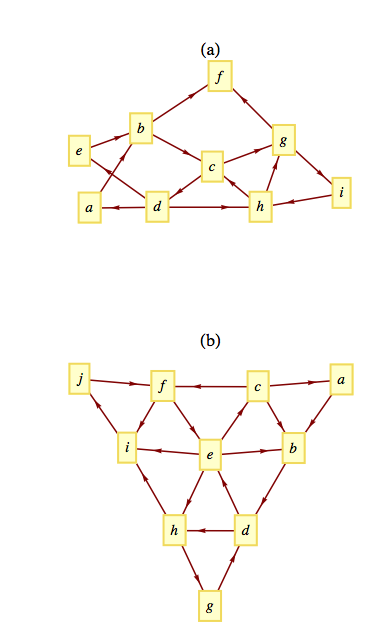
\includegraphics[width=1\linewidth]{images/fig-exercise-9-3-4.png}
\end{figure}
\par\smallskip
\end{exercisegroup}
\par\smallskip\noindent
\hypertarget{exercisegroup-4}{}\typeout{************************************************}
\typeout{Introduction  }
\typeout{************************************************}
B Exercises%
\begin{exercisegroup}
\item[5.]\hypertarget{exercise-20}{} Prove (by induction on \(k\)) that if the relation \(r\) on vertices of a graph is defined by \(v r w\) if there is an edge connecting
\(v\) to \(w\), then \(r^k\) ,\(k \geq  1\), is defined by \(v r^kw\) if there is a path of length \(k\) from \(v\) to
\(w\).%
\par\smallskip
\par\smallskip
\noindent\textbf{Answer.}\hypertarget{answer-5}{}\quad
 Basis: \((k=1)\) Is the relation \(r^1\)defined by \(\text{\textit{vr}}^1w\) if there is a path of length \(l\) from \(v \text{to} w\)? Yes, since
\textit{ \(\text{vrw}\)} if and only if an edge, which is a path of length \(l\), connects \(v\) to \(w\).%
\par
Induction: Assume that \(\text{\textit{vr}}^kw\) if and only if there is a path of length \textit{ k }from \(v\) to \(w\). We must show
that \(\text{\textit{vr}}^{k+1}w\) if and only if there is a path of length \(k+1\) from \(v\) to \(w\).%
\par

\(\text{\textit{vr}}^{k+1}w\Rightarrow \text{\textit{vr}}^ky \text{and} \text{\textit{yrw}}\), for some vertex \(y\). By the induction
hypothesis, there is a path of length \(k\) from \(v \text{to} y\). And by the basis, there is a path of length one from \(y\) to \textit{
w}. If we combine these two paths, we obtain a path of length \(k+1\) from \(v\) to \(w\). Of course, if we start with a path of length
\(k+1\) from \(v\) to \(w\), we have a path of length \(k\) from \(v\) to some vertex \(y\) and a path of length\textit{
 l} from \(y\) to \(w\). Therefore, \(\text{\textit{vr}}^ky \text{and} \text{\textit{yrw}}\Rightarrow \text{\textit{vr}}^{k+1}w\text{
   }\square\)
%
\end{exercisegroup}
\par\smallskip\noindent
\typeout{************************************************}
\typeout{Section 1.4 Traversals: Eulerian and Hamiltonian Graphs}
\typeout{************************************************}
\section[Traversals: Eulerian and Hamiltonian Graphs]{Traversals: Eulerian and Hamiltonian Graphs}\label{s-traversals}
\index{Traversals of Graphs}\typeout{************************************************}
\typeout{Introduction  }
\typeout{************************************************}
The subject of graph traversals has a long history. In fact, the solution by Leonhard Euler (Switzerland, 1707-83) of the Koenigsberg Bridge
Problem is considered by many to represent the birth of graph theory.%
\typeout{************************************************}
\typeout{Subsection 1.4.1 Eulerian  Graphs}
\typeout{************************************************}
\subsection[Eulerian  Graphs]{Eulerian  Graphs}\label{ss-eulerian}
% group protects changes to lengths, releases boxes (?)
{% begin: group for a single side-by-side
% set panel max height to practical minimum, created in preamble
\setlength{\panelmax}{0pt}
\newsavebox{\panelboxQimage}
\savebox{\panelboxQimage}{
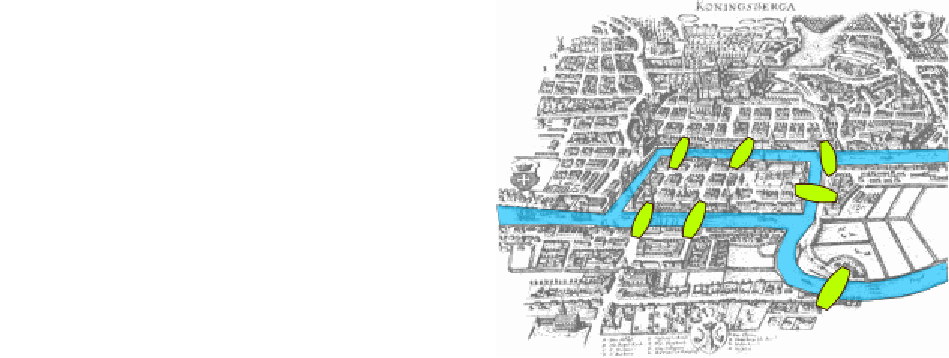
\includegraphics[width=0.5\linewidth]{images/fig-konigsberg-map.png}
}
\newlength{\phQimage}\setlength{\phQimage}{\ht\panelboxQimage+\dp\panelboxQimage}
\settototalheight{\phQimage}{\usebox{\panelboxQimage}}
\setlength{\panelmax}{\maxof{\panelmax}{\phQimage}}
\newsavebox{\panelboxRimage}
\savebox{\panelboxRimage}{
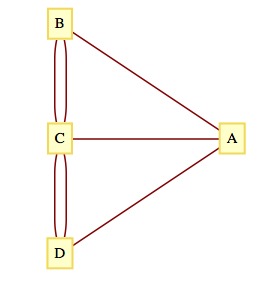
\includegraphics[width=0.5\linewidth]{images/fig-konigsberg-multigraph.png}
}
\newlength{\phRimage}\setlength{\phRimage}{\ht\panelboxRimage+\dp\panelboxRimage}
\settototalheight{\phRimage}{\usebox{\panelboxRimage}}
\setlength{\panelmax}{\maxof{\panelmax}{\phRimage}}
\leavevmode%
% begin: side-by-side as figure/tabular
% \tabcolsep change local to group
\setlength{\tabcolsep}{0\textwidth}
% @{} suppress \tabcolsep at extremes, so margins behave as intended
\begin{figure}
\begin{tabular}{@{}*{2}{c}@{}}
\begin{minipage}[c][\panelmax][t]{0.5\textwidth}\usebox{\panelboxQimage}\end{minipage}&
\begin{minipage}[c][\panelmax][t]{0.5\textwidth}\usebox{\panelboxRimage}\end{minipage}\tabularnewline
\parbox[t]{0.5\textwidth}{\subcaption{A  map of Koenigsberg, circa 1735 \label{fig-konigsberg-map}}
}&
\parbox[t]{0.5\textwidth}{\subcaption{A multigraph for the bridges of Koenigsberg\label{fig-konigsberg-multigraph}}
}\end{tabular}
\caption{The Koenigsberg Bridge Problem\label{fig-sidebyside-konigsberg}}
\end{figure}
% end: side-by-side as tabular/figure
}% end: group for a single side-by-side
A map of the Prussian city of Koenigsberg (circa 1735) in Figure 9.4.1 shows that there were seven bridges connecting the four land masses that
made up the city. The legend of this problem states that the citizens of Koenigsberg searched in vain for a walking tour that passed over each
bridge exactly once. No one could design such a tour and the search was abruptly abandoned with the publication of Euler's Theorem.%
\begin{theorem}[Euler's Theorem - Koenigsberg Case]\label{th-euler-theorem-koenigsberg-case}
\index{Euler's Theorem!Koenigsberg Case}No walking tour of \(K\"onigsberg\) can be designed so that each bridge is used exactly
once.%
\end{theorem}
\begin{proof}\hypertarget{proof-2}{}
The map of Koenigsberg can be represented as an undirected multigraph, as in Figure 9.4.2. The four land masses are the vertices and each
edge represents a bridge. %
\par
The desired tour is then a path that uses each edge once and only once. Since the path can start and end at two different
vertices, there are two remaining vertices that must be intermediate vertices in the path. If \(x\) is an intermediate vertex, then every time
that you visit \(x\), you must use two of its incident edges, one to enter and one to exit. Therefore, there must be an even number of edges
connecting \(x\) to the other vertices. Since every vertex in the Koenigsberg graph has an odd number of edges, no tour of the type that
is desired is possible. %
\end{proof}
\par
As is typical of most mathematicians, Euler wasn't satisfied with solving only the Koenigsberg problem. His original theorem, which is paraphrased
below, concerned the existence of paths and circuits like those sought in Koenigsberg. These paths and circuits have become associated with Euler's
name.%
\begin{definition}[Eulerian Paths, Circuits, Graphs.]\label{def-eulerian-paths-circuits-graphs}
\index{Eulerian Paths, Circuits, Graphs.} A Eulerian path through a graph is a path whose edge list contains each edge of the graph exactly
once. If the path is a circuit, then it is called a Eulerian circuit. A Eulerian graph is a graph that possesses a Eulerian path.%
\end{definition}
\begin{example}[An Eulerian Graph]\label{ex-an-eulerian-graph}
Without tracing any paths, we can be sure that the graph below has an Eulerian circuit because all vertices have an even
degree. This follows from the following theorem.
%
\leavevmode%
\begin{figure}
\centering
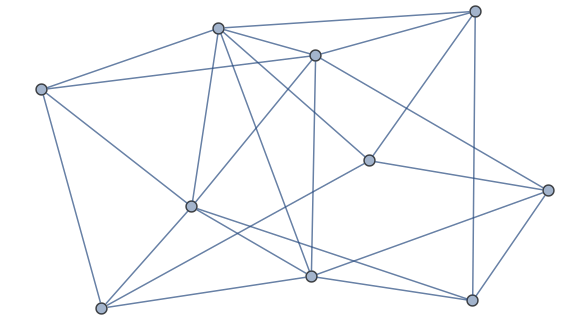
\includegraphics[width=1\linewidth]{images/fig-eulerian-9-4.png}
\caption{An Eulerian graph
                \label{fig-eulerian-9-4}}
\end{figure}
\end{example}
\begin{theorem}[Euler's Theorem - General Case]\label{theorem-euler-theorem-general}
\index{Euler's Theorem}An undirected graph is Eulerian if and only if it is connected and has either zero or two vertices with an odd degree. If no vertex has an odd degree, then the graph has a Eulerian circuit.%
\end{theorem}
\begin{proof}\hypertarget{proof-3}{}
It can be proven by induction that the number of vertices in an undirected graph that have an odd degree must be even. We will leave
the proof of this fact to the reader as an exercise. The necessity of having either zero or two vertices of odd degree is clear from the proof of
the Koenigsberg case of this theorem. Therefore, we will concentrate on proving that this condition is sufficient to ensure that a graph is Eulerian.
Let \(k\) be the number of vertices with odd degree.%
\par
 Phase 1. If \(k = 0\), start at any vertex, \(v_0\), and travel along any path, not using any edge twice. Since each vertex has an even
degree, this path can always be continued past each vertex that you reach except \(v_0\). The result is a circuit that includes \(v_0\). If \(k =
2\), let \(v_0\) be either one of the vertices of odd degree. Trace any path starting at \(v_0\) using up edges until you can go no further, as in
the \(k = 0\) case. This time, the path that you obtain must end at the other vertex of odd degree that we will call \(v_1\).  At the end of Phase
1, we have an initial path that may or may not be Eulerian. If it is not Eulerian, Phase 2 can be repeated until all of the edges have been used.
Since the number of unused edges is decreased in any use of Phase 2, a Eulerian path must be obtained in a finite number of steps.%
\par
 Phase 2. As we enter this phase, we have constructed a path that uses a proper subset of the edges in our graph. We will refer to this
path as the current path. Let \(V\) be the vertices of our graph, \(E\) the edges, and \(E_u\) the edges that have been used in the current
path. Consider the graph \(G' = \left(V, E - E_u\right)\).  Note that every vertex in \(G'\) has an even degree. Select any edge, \textit{
e}, from \(G'.\) Let \(v_a\) and \(v_b\) be the vertices that \(e\) connects. Trace a new path starting at \(v_a\) whose first edge is \textit{
e}. We can be sure that at least one vertex of the new path is also in the current path since \((V, E)\) is connected. Starting at \(v_a\), there
exists a path in \((V, E)\) to any vertex in the current path. At some point along this path, which we can consider the start of the new path, we
will have intersected the current path. Since the degree of each vertex in G' is even, any path that we start at \(v_a\) can be continued until it
is a circuit. Now, we simply augment the current path with this circuit. As we travel along the current path, the first time that we intersect the
new path, we travel along it (see Figure 9.4.3). Once we complete the circuit that is the new path, we resume the traversal of the current path.%
\leavevmode%
\begin{figure}
\centering
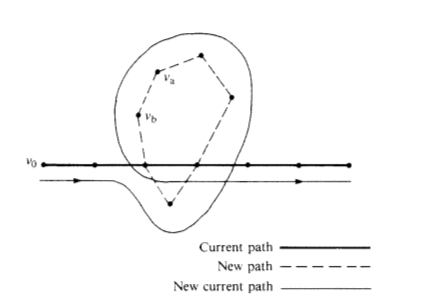
\includegraphics[width=1\linewidth]{images/fig-path-augmentation.png}
\caption{Path Augmentation Plan
                \label{fig-path-augmentation}}
\end{figure}
\par
If the result of this phase is a Eulerian path, then we are finished; otherwise, repeat this phase.%
\end{proof}
\begin{example}[Complete Eulerian Graphs]\label{ex-complete-eulerian}
The complete undirected graphs \(K_2\) and \(K_{2n+1}\), \(n = 1, 2, 3, \ldots\). .., are Eulerian. If \(n>1\), then \(K_{2n}\)
is not Eulerian.
%
\end{example}
\typeout{************************************************}
\typeout{Subsection 1.4.2 Hamiltonian Graphs}
\typeout{************************************************}
\subsection[Hamiltonian Graphs]{Hamiltonian Graphs}\label{ss-hamiltonian-graphs}
To search for a path that uses every vertex of a graph exactly once seems to be a natural next problem after you have considered Eulerian graphs.The Irish mathematician Sir William Rowan Hamilton (1805-65) is given credit for first defining such paths. He is also credited with discovering the quaternions, for which he was honored by the Irish government with a postage stamp in 2004.%
\leavevmode%
\begin{figure}
\centering
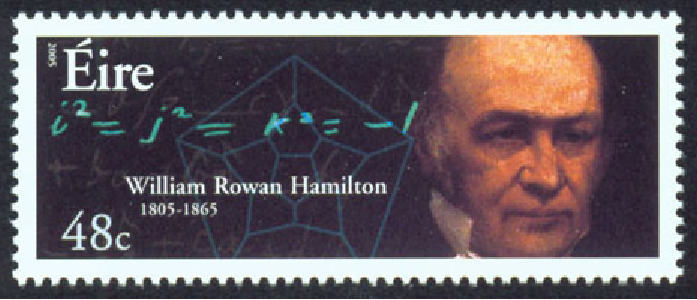
\includegraphics[width=1\linewidth]{images/fig-hamilton-stamp.png}
\caption{Irish stamp honoring Sir William Rowan Hamilton
                \label{fig-hamilton-stamp}}
\end{figure}
\begin{definition}[Hamiltonian Path, Circuit, and Graphs]\label{def-hamiltonian-path-circuit-graph}
\index{Hamiltonian Paths, Circuits, and Graphs}A Hamiltonian path through a graph is a path whose vertex list contains each vertex of the graph exactly once, except if the path is a circuit, in which case the initial vertex appears a second time as the terminal vertex. If the path is a circuit, then it is called a Hamiltonian circuit. A Hamiltonian graph is a graph that possesses a Hamiltonian path.%
\end{definition}
\begin{example}[The Original Hamiltonian Graph]\label{ex-dodec-graph}
\hyperref[fig-dodec-graph]{Figure~\ref{fig-dodec-graph}} shows a graph that is Hamiltonian. In fact, it is the graph that Hamilton used as an example to pose the question of existence of Hamiltonian paths in 1859. In its original form, the puzzle that was posed to readers was called ``Around the World.'' The vertices were labeled with names of major cities of the world and the object was to complete a tour of these cities. The graph is also referred to as the
dodecahedron graph, where vertices correspond with the corners of a dodecahedron and the edges are the edges of the solid that connect the corners.%
% group protects changes to lengths, releases boxes (?)
{% begin: group for a single side-by-side
% set panel max height to practical minimum, created in preamble
\setlength{\panelmax}{0pt}
\newsavebox{\panelboxVimage}
\savebox{\panelboxVimage}{
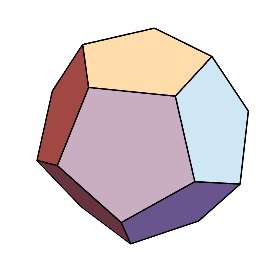
\includegraphics[width=0.5\linewidth]{images/fig-dodec.png}
}
\newlength{\phVimage}\setlength{\phVimage}{\ht\panelboxVimage+\dp\panelboxVimage}
\settototalheight{\phVimage}{\usebox{\panelboxVimage}}
\setlength{\panelmax}{\maxof{\panelmax}{\phVimage}}
\newsavebox{\panelboxWimage}
\savebox{\panelboxWimage}{
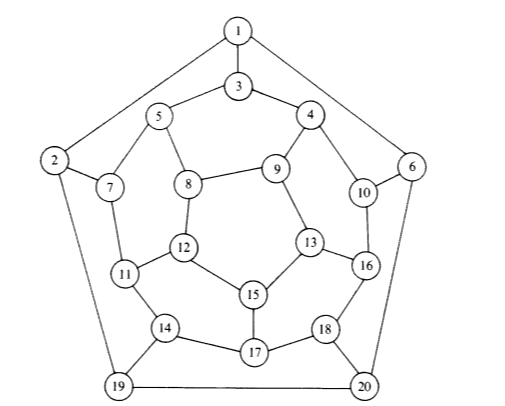
\includegraphics[width=0.5\linewidth]{images/fig-dodec-graph.png}
}
\newlength{\phWimage}\setlength{\phWimage}{\ht\panelboxWimage+\dp\panelboxWimage}
\settototalheight{\phWimage}{\usebox{\panelboxWimage}}
\setlength{\panelmax}{\maxof{\panelmax}{\phWimage}}
\leavevmode%
% begin: side-by-side as figure/tabular
% \tabcolsep change local to group
\setlength{\tabcolsep}{0\textwidth}
% @{} suppress \tabcolsep at extremes, so margins behave as intended
\begin{figure}
\begin{tabular}{@{}*{2}{c}@{}}
\begin{minipage}[c][\panelmax][t]{0.5\textwidth}\usebox{\panelboxVimage}\end{minipage}&
\begin{minipage}[c][\panelmax][t]{0.5\textwidth}\usebox{\panelboxWimage}\end{minipage}\tabularnewline
\parbox[t]{0.5\textwidth}{\captionof{figure}{A Dodecahedron\label{fig-dodec}}
}&
\parbox[t]{0.5\textwidth}{\captionof{figure}{The Dodecahedron Graph\label{fig-dodec-graph}}
}\end{tabular}
\end{figure}
% end: side-by-side as tabular/figure
}% end: group for a single side-by-side
\end{example}
\begin{problem}[]\label{problem-1}
Unfortunately, a simple condition doesn't exist that characterizes a Hamiltonian graph. An obvious necessary condition is that the
graph be connected; however, there is a connected undirected graph with four vertices that is not Hamiltonian. Can you draw such a graph? 
%
\end{problem}
\begin{note}[A Note on What Is Possible and What Is Impossible]\label{note-5}
The search for a Hamiltonian path in a graph is typical of many simple-sounding problems
in graph theory that have proven to be very difficult to solve. Although there are simple algorithms for conducting the search, they are impractical
for large problems because they take such a long time to complete as graph size increases. Currently, every algorithm to search for a Hamiltonian
path in a graph takes exponential time to complete. That is, if \(T(n)\) is the time it takes to search a graph of \(n\) vertices, then there
is a positive real number \(a\), \(a > 1\), such that \(T(n) > a^n\) for all but possibly a finite number of positive values for \textit{
n}. No matter how close to 1 we can make \(a\), \(a^n\) will grow at such a fast rate that the algorithm will not be feasible for large values
of \(n\). For a given algorithm, the value of a depends on the relative times that are assigned to the steps, but in the search for Hamiltonian
paths, the actual execution time for known algorithms is large with 20 vertices. For 1,000 vertices, no algorithm is likely to be practical, and
for 10,000 vertices, no currently known algorithm could be executed.%
\par
It is an unproven but widely held belief that no faster algorithm exists to search for Hamiltonian paths in general groups. A faster algorithm would have to be one
that takes only polynomial time; that is, \(T(n) < p(n)\), for some polynomial sequence \(p\). To sum up, the problem of determining whether
a graph is Hamiltonian is theoretically possible; however, for large graphs we consider it a practical impossibility. Many of the problems we will discuss in the next section, particularly the Traveling Salesman Problem, are thought to be impossible in the same sense. 
%
\end{note}
\begin{definition}[The \(n\)-cube.]\label{def-n-cube}
\index{N-cube}\label{notation-4}
Let \(n \geq  1\), and let \(B^n\) be the set of strings of 0's and 1's with length n.  The \(n\)-cube is the undirected graph with a vertex for each string in \(B^n\) and an edge connecting each pair of strings that differ in exactly one position. The \(n\)-cube is normally denoted \(Q_n\). %
\end{definition}
\par
The \(n\)-cube is among the graphs that are defined within the \lstinline?graphs? package of Sage and is created with the expresson \lstinline?graphs.CubeGraph(n)?. %
\begin{lstlisting}[style=sageinput]
graphs.CubeGraph(4).show()
\end{lstlisting}
\begin{note}[The Gray Code]\label{note-gray-code}
 A Hamiltonian circuit of the \(n\)-cube can be described recursively. The circuit itself, called the Gray Code, is
not the only Hamiltonian circuit of the \(n\)-cube, but it is the easiest to describe. The standard way to write the Gray Code is as a column of strings, where the last string is followed by the first string to complete the circuit.%
\par
Basis for the Gray Code (\(n = 1\)): The Gray Code for the 1-cube is \(G_1=\left(
\begin{array}{c}
 0 \\
 1 \\
\end{array}
\right)\).  Note that the edge between 0 and 1 is used twice in this circuit. That doesn't violate any rules for Hamiltonian circuits, but
can only happen if a graph as two vertices.%
\par
Recursive definition of the Gray Code: Given the Gray Code for the \(n\)-cube, \(n > 1\), then \(G_{n+1}\) is obtained by (1) listing \(G_n\) with each string prefixed
with 0, and then (2) reversing the list of strings in \(G_n\) with each string prefixed with 1. Symbolically, the recursion can
be expressed as



\[G_{n+1}=\left(
\begin{array}{c}
 0 G_n \\
 1 G_n^r \\
\end{array}
\right)\]



where \(G_n^r\) is the reverse of list \(G_n\).%
\par
The Gray Codes for the 2-cube and 3-cube are

\[G_2= \left(
\begin{array}{c}
 00 \\
 01 \\
 11 \\
 10 \\
\end{array}
\right) \textrm{  and   }G_3=\left(
\begin{array}{c}
 000 \\
 001 \\
 011 \\
 010 \\
 110 \\
 111 \\
 101 \\
 100 \\
\end{array}
\right)\]
%
\end{note}
\begin{example}[Applications of the Gray Code]\label{example-16}
 One application of the Gray code was discussed in the Introduction to this book.  An other application is
in statistics. In a statistical analysis, there is often a variable that depends on several factors, but exactly which factors are significant
may not be obvious. For each subset of factors, there would be certain quantities to be calculated. One such quantity is the multiple correlation
coefficient for a subset. If the correlation coefficient for a given subset, \(A\), is known, then the value for any subset that is obtained
by either deleting or adding an element to \(A\) can be obtained quickly. To calculate the correlation coefficient for each set, we simply
travel along \(G_n\), where \(n\) is the number of factors being studied. The first vertex will always be the string of 0's, which represents
the empty set. For each vertex that you visit, the set that it corresponds to contains the \(k^{\text{th}}\) factor if the \(k^{\text{th}}\) character
is a 1.%
\end{example}
\typeout{************************************************}
\typeout{Exercises 1.4.3 Exercises for Section 9.4}
\typeout{************************************************}
\subsection[Exercises for Section 9.4]{Exercises for Section 9.4}\label{exercises-9-4}
\hypertarget{exercisegroup-5}{}\typeout{************************************************}
\typeout{Introduction  }
\typeout{************************************************}
A Exercises%
\begin{exercisegroup}
\item[1.]\hypertarget{exercise-21}{} Locate a map of New York City and draw a graph that represents its land masses, bridges and tunnels. Is there a Eulerian path through New York? You can do the same with any other city that has at least two land masses.%
\par\smallskip
\par\smallskip
\noindent\textbf{Answer.}\hypertarget{answer-6}{}\quad
 Using a recent road map, it appears that a Eulerian circuit exists in New York City, not including the small islands that belong to the city.
Lowell, Massachusetts, is located at the confluence of the Merrimack and Concord rivers and has several canals flowing through it. No Eulerian path
exists for Lowell.

%
\item[2.]\hypertarget{exercise-22}{} Which of the drawings in \hyperref[fig-drawings-9-4]{Figure~} can be drawn without removing your pencil from the paper and without drawing any line twice?%
\leavevmode%
\begin{figure}
\centering
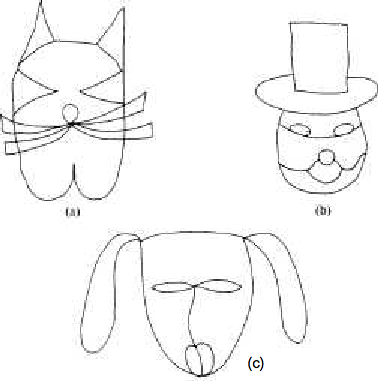
\includegraphics[width=1\linewidth]{images/fig-drawings-9-4.png}
\end{figure}
\par\smallskip
\item[3.]\hypertarget{exercise-23}{}Write out the Gray Code for the 4-cube.%
\par\smallskip
\par\smallskip
\noindent\textbf{Answer.}\hypertarget{answer-7}{}\quad
 Gray Code for the 4-cube:
\[G_4=\left(
\begin{array}{c}
 0000 \\
 0001 \\
 0011 \\
 0010 \\
 0110 \\
 0111 \\
 0101 \\
 0100 \\
 1100 \\
 1101 \\
 1111 \\
 1110 \\
 1010 \\
 1011 \\
 1001 \\
 1000 \\
\end{array}
\right)\]
%
\item[4.]\hypertarget{exercise-24}{} Find a Hamiltonian circuit for the dodecahedron graph in \hyperref[fig-dodec-graph]{Figure~\ref{fig-dodec-graph}}.%
\par\smallskip
\item[5.]\hypertarget{exercise-25}{} The Euler Construction Company has been contracted to construct an extra bridge in Koenigsberg so that a Eulerian path through the town
exists. Can this be done, and if so, where should the bridge be built?%
\par\smallskip
\par\smallskip
\noindent\textbf{Answer.}\hypertarget{answer-8}{}\quad
 Any bridge between two land masses will be sufficient. To get a Eulerian circuit, you must add a second bridge that connects the two land masses
that were not connected by the first bridge.
%
\item[6.]\hypertarget{exercise-26}{}\leavevmode%
\begin{enumerate}[label=\alph*]
\item\hypertarget{li-63}{}Determine which of the graphs in Figure 9.4.8 has a Eulerian path?%
\item\hypertarget{li-64}{}Find a Eulerian path for the graphs that have one.%
\end{enumerate}
%
\leavevmode%
\begin{figure}
\centering
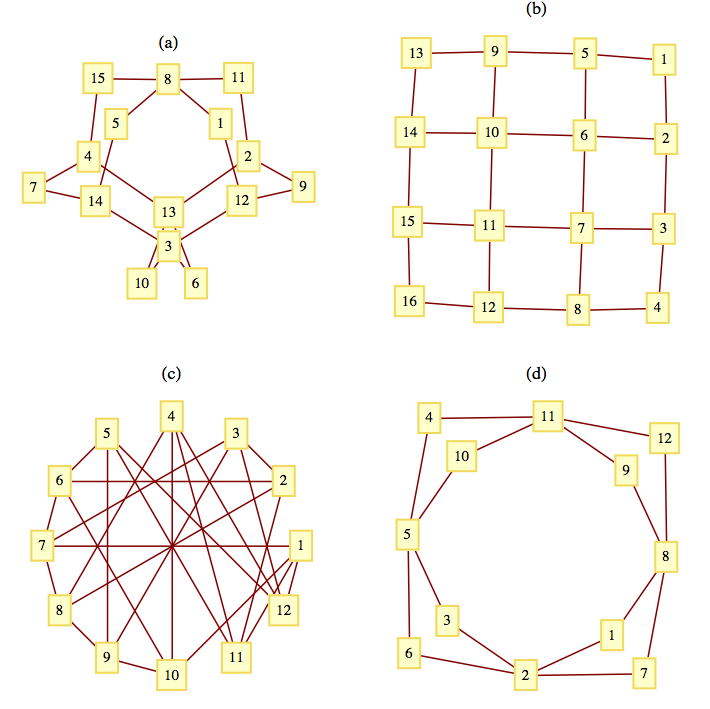
\includegraphics[width=1\linewidth]{images/fig-exercise-9-4-6.png}
\end{figure}
\par\smallskip
\end{exercisegroup}
\par\smallskip\noindent
\hypertarget{exercisegroup-6}{}\typeout{************************************************}
\typeout{Introduction  }
\typeout{************************************************}
B Exercises%
\begin{exercisegroup}
\item[7.]\hypertarget{exercise-27}{} Formulate Euler's theorem for directed graphs.%
\par\smallskip
\par\smallskip
\noindent\textbf{Answer.}\hypertarget{answer-9}{}\quad
Let  \(G=(V,E)\)} be a directed graph. \(G\) has a Eulerian circuit if and only if G is connected and (\text{indeg}(v)=\text{outdeg}(v)\) for all \(v\) in \(V\). There exists a Eulerian path from  \(v_1\textrm{ to } v_2\)  if and only if 
g is connected, \(\text{indeg}\left(v_1\right)=\text{outdeg}\left(v_1\right)-1\), \(\text{indeg}\left(v_2\right)=\text{outdeg}\left(v_2\right)+1\),
 and for all other vertices in \(V\) the indegree and outdegree are equal.%
\item[8.]\hypertarget{exercise-28}{} Prove that the number of vertices in an undirected graph with odd degree must be even.%
\par\smallskip
\par\smallskip
\noindent\textbf{Hint.}\hypertarget{hint-1}{}\quad
 Prove by induction on the number of edges.%
\item[9.]\hypertarget{exercise-29}{}\leavevmode%
\begin{enumerate}[label=\alph*]
\item\hypertarget{li-65}{}Under what conditions will a round-robin tournament graph be Eulerian?%
\item\hypertarget{li-66}{}Prove that every round-robin tournament graph is Hamiltonian.%
\end{enumerate}
%
\par\smallskip
\par\smallskip
\noindent\textbf{Answer.}\hypertarget{answer-10}{}\quad
 A round-robin tournament graph is rarely Eulerian. It will be Eulerian if it has an odd number of vertices and each vertex (team) wins exactly
as many times as it loses. Every round-robin tournament graph has a Hamiltonian path. This can be proven by induction on the number of vertices.%
\item[10.]\hypertarget{exercise-30}{} For what values of \(n\) is  n-cube Eulerian.%
\par\smallskip
\end{exercisegroup}
\par\smallskip\noindent
\typeout{************************************************}
\typeout{Section 1.5 Graph Optimization}
\typeout{************************************************}
\section[Graph Optimization]{Graph Optimization}\label{s-graph-optimization}
\index{Graph Optimization}\typeout{************************************************}
\typeout{Introduction  }
\typeout{************************************************}
The common thread that connects all of the problems in this section is the desire to optimize (maximize or minimize) a quantity that is associated with a graph. We will concentrate most of our attention on two of these problems, the Traveling Salesman Problem and the Maximum Flow Problem. At the close of this section, we will discuss some other common optimization problems.%
\typeout{************************************************}
\typeout{Subsection 1.5.1 Weighted Graphs}
\typeout{************************************************}
\subsection[Weighted Graphs]{Weighted Graphs}\label{ss-weighted-graph}
\begin{definition}[Weighted Graph]\label{def-weighted-graph}
\index{Weighted Graph}A weighted graph, \((V, E, w)\), is a graph \((V, E)\) together with a weight function \(w: E \to \mathbb{R}\).
If \(e \in  E\), \(w(e)\) is the weight on edge e.%
\end{definition}
As you will see in our examples, \(w(e)\) is often a cost associated with the edge e; therefore, most weights will be positive.%
\begin{example}[A Distance Graph]\label{ex-distance-graph}
Let V be the set of six capital cities in New England: Boston, Augusta, Hartford, Providence, Concord, and Montpelier. Let \(E\) be \(\{\{a, b\} \in  V \times V| a\neq  b\}\); that is, \((V,E)\) is a complete unordered graph. An example of a weight function on this graph is \(w\left(c_1, c _2\right) = \textrm{the distance, in miles, from } c_1 \textrm{ to } c_2\). %
\par
Many road maps define distance functions as in the following table.%
\leavevmode%
\begin{table}
\centering
\begin{tabular}{ccccccc}\hrulethick
--&Augusta&Boston&Concord&Hartford&Montpelier&Providence\tabularnewline[0pt]
Augusta, ME&--&165&148&266&190&208\tabularnewline[0pt]
Boston, MA&165&--&75&103&192&43\tabularnewline[0pt]
Concord, NH&148&75&--&142&117&109\tabularnewline[0pt]
Hartford, CT&266&103&142&--&204&70\tabularnewline[0pt]
Montpelier, VT&190&192&117&204&--&223\tabularnewline[0pt]
Providence, RI&208&43&109&70&223&--
\end{tabular}
\caption{Distances between capital cities in New England\label{table-ne-capitals}}
\end{table}
\end{example}
\typeout{************************************************}
\typeout{Subsection 1.5.2 The Traveling Salesman Problem}
\typeout{************************************************}
\subsection[The Traveling Salesman Problem]{The Traveling Salesman Problem}\label{ss-traveling-salesman-problem}
\index{The Traveling Salesman Problem}The Traveling Salesman Problem is, given a weighted graph, to find a circuit \(\left(e_1, e_2,\ldots ,e_n\right)\) that visits every vertex at least once and minimizes the sum of the weights, \(\sum_{i=1}^n w\left(e_i\right)\).  Any such circuit is called an  optimal path.%
\par
Some statements of the Traveling Salesman Problem require that the circuit be Hamiltonian. In many applications, the graph in question
will be complete and this restriction presents no problem.  If the weight on each edge is constant, for example, \(w(e) = 1\), then an optimal path would be any Hamiltonian circuit.%
\begin{example}[The problem of a Boston salesman]\label{ex-boston-salesman}
 The Traveling Salesman Problem gets its name from the situation of a salesman who wants to minimize the number of miles that
he travels in visiting his customers. For example, if a salesman from Boston must visit the other capital cities of New England, then the problem is to find a circuit in the weighted graph of \hyperref[ex-distance-graph]{Example~\ref{ex-distance-graph}}. Note that distance and cost are clearly related in this case. In addition, tolls and traffic congestion might also be taken into account. 
%
\end{example}
\par
The search for an efficient algorithm that solves the Traveling Salesman has occupied researchers for years. If the graph in question is complete,
there are \((n -1)!\) different circuits. As \(n\) gets large, it is impossible to check every possible circuit. The most efficient algorithms
for solving the Traveling Salesman Problem take an amount of time that is proportional to \(n 2^n\). Since this quantity grows so quickly, we can't
expect to have the time to solve the Traveling Salesman Problem for large values of \(n\). Most of the useful algorithms that have been developed
have to be heuristic; that is, they find a circuit that should be close to the optimal one. One such algorithm is the ``closest neighbor'' algorithm,
one of the earliest attempts at solving the Traveling Salesman Problem. The general idea behind this algorithm is, starting at any vertex, to visit
the closest neighbor to the starting point. At each vertex, the next vertex that is visited is the closest one that has not been reached. This shortsighted
approach typifies heuristic algorithms called  greedy algorithms, which attempt to solve a minimization (maximization) problem
by minimizing (maximizing) the quantity associated with only the first step.%
\begin{algorithm}[The Closest Neighbor Algorithm]\label{alg-closest-neighbor}
\index{Closest Neighbor Algorithm}Let \(G = (V, E, w)\) be a complete weighted graph with \(|V| = n\). The closest neighbor
circuit through G starting at \(v_1\) is \(\left(v_1, v_2,\ldots ,v_n\right)\), defined by the steps:%
\par
\leavevmode%
\begin{enumerate}[label=\arabic*]
\item\hypertarget{li-67}{} \(V_1= V-\left\{v_1\right\}\).%
\item\hypertarget{li-68}{}For \(k\text{  }= 2  \textrm{ to } n - 1\) %
\par
%
\begin{enumerate}[label=\alph*]
\item\hypertarget{li-69}{} \(v_k= \textrm{ the closest vertex in } V_{k-1} \textrm{ to }
						 v_{k-1}\):
	 \[w\left(v_{k-1} , v _k\right) = \min  \left(w\left(v_{k-1} ,v\right) \mid v \in  V_{k-1}\right)\] 
 In case of a tie for closest, \(v_k\) may be chosen arbitrarily.%
\item\hypertarget{li-70}{} \(V_k= V_{k-1} - \left\{v_k \right\}\)%
\end{enumerate}
%
\item\hypertarget{li-71}{}\(v_n= \textrm{the only element of } V_n\)%
\end{enumerate}
%
\par
The cost of the closest neighbor circuit is
\(\sum_{k=1}^{n-1} w\left(v_k,v_{k+1}\right)+w\left(v_n,v_1\right)\)%
\end{algorithm}
\begin{example}[A small example]\label{ex-tsp-small-example}
 The closest neighbor circuit starting at A in Figure 9.5.2 is \((1,3,2,4,1)\), with a cost of 29. The optimal path is \((1,2,3,4,1)\),
with a cost of 27.%
\leavevmode%
\begin{figure}
\centering
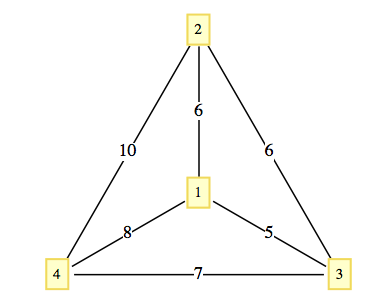
\includegraphics[width=1\linewidth]{images/fig-small-tsp-example.png}
\end{figure}
\end{example}
\par
Although the closest neighbor circuit is often not optimal, we may be satisfied if it is close to optimal. If \(C_{\text{opt}}\) and \(C_{\text{cn}}\)
are the costs of optimal and closest neighbor circuits in a graph, then it is always the case that \(C_{\text{opt}}\leq C_{\text{cn}}\) or \(\frac{C_{\text{cn}}}{C_{\text{opt}}}\geq
1\). We can assess how good the closest neighbor algorithm is by determining how small the quantity \(\frac{C_{\text{cn}}}{C_{\text{opt}}}\) gets.
If it is always near 1, then the algorithm is good. However, if there are graphs for which it is large, then the algorithm may be discarded. Note
that in \hyperref[ex-tsp-small-example]{Example~\ref{ex-tsp-small-example}}, \(\frac{C_{\text{cn}}}{C_{\text{opt}}} = \frac{29}{27}\approx 1.074\). A 7 percent increase in cost may or may not be considered
significant, depending on the situation.%
\begin{example}[The One-way Street]\label{ex-one-way-street}
 A salesman must make stops at vertices A, B, and C, which are all on the same one-way street. The graph in Figure \hyperref[fig-directed-tsp-example]{Figure~} is weighted by the function \(w(i, j)\) equal to the time it takes to drive from vertex \(i\) to vertex \(j\).%
\leavevmode%
\begin{figure}
\centering
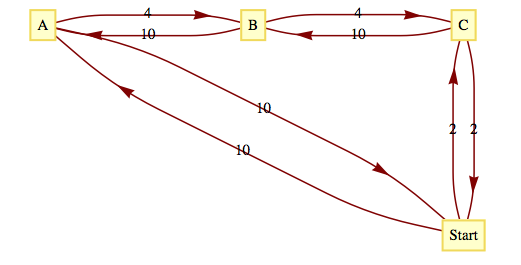
\includegraphics[width=1\linewidth]{images/fig-directed-tsp-example.png}
\end{figure}
\par
Note that if \(j\) is down the one-way street from \(i\), then \(w(i, j) &lt; w(j, i)\). The values of \(C_{\text{opt}}\) , and \(C_{\text{cn}}\)
are 20 and 32, respectively. Verify that \(C_{\text{cn}}\) is 32 by using the closest neighbor algorithm. The value of \(\frac{C_{\text{cn}}}{C_{\text{opt}}} = 1.6\) is significant in this case since our salesman would spend 60 percent more time on the road if he used the closest neighbor algorithm.%
\end{example}
\par
A more general result relating to the closest neighbor algorithm presumes that the graph in question is complete and that the weight function satisfies the conditions%
\par
\leavevmode%
\begin{itemize}[label=\textbullet]
\item{} \(w(x, v) = w(y, x)\) for all  x, y in the vertex set, and %
\item{} \(w(x, y) + w(y, z) \geq  w(x, z)\) for all  x, y, z in the vertex set.%
\end{itemize}
%
\par
The first condition is called the  symmetry condition and the second is the  triangle inequality.%
\begin{theorem}[]\label{th-cn-theorem-9-5}
\index{}If \((V, E, w)\) is a complete weighted graph that satisfies the symmetry and triangle inequality conditions, then
\[\frac{C_{\text{cn}}}{C_{\text{opt}}}\leq \frac{\left\lceil \log _2 (2n)\right\rceil }{2}\]%
\end{theorem}
\begin{observation}[]\label{observation-1}
If \(|V|=8\), then this theorem says that \(C_{\text{cn}}\) can be no larger than twice the size of \(C_{\text{opt}}\); however,
it doesn't say that the closest neighbor circuit will necessarily be that far from an optimal circuit. The quantity \(\frac{\left\lceil \log _2 (2n)\right\rceil
}{2}\) is called an upper bound for the ratio \(\frac{C_{\text{cn}}}{C_{\text{opt}}}\). It tells us only that things can't be any worse than the
upper bound. Certainly, there are many graphs with eight vertices such that the optimal and closest neighbor circuits are the same. What is left
unstated in this theorem is whether there are graphs for which the quantities are equal. If there are such graphs, we say that the upper
bound is  sharp.%
\par
 The value of \(\frac{C_{\text{cn}}}{C_{\text{opt}}}\) in Example \hyperref[ex-one-way-street]{\ref{ex-one-way-street}} is 1.6, which is greater than \(\frac{\left\lceil \log _2 (2\ 4)\right\rceil
}{2} = 1.5\); however, the weight function in this example does not satisfy the conditions of the theorem.%
\end{observation}
\begin{example}[The Unit Square Problem]\label{ex-unit-square}
Suppose a robot is programmed to weld joints on square metal plates. Each plate must be welded at prescribed points on the square.
To minimize the time it takes to complete the job, the total distance that a robot's arm moves should be minimized. Let \(d(P, Q)\) be the distance
between \(P\) and \(Q\). Assume that before each plate can be welded, the arm must be positioned at a certain point \(P_0\) . Given
a list of \(n\) points, we want to put them in order so that



      \[d\left(P _0,P_1\right) + d\left(P_1,P _2 \right) +\cdots +d\left(P_{n-1},P_n\right)+ d\left(P_n ,P _0 \right)\]

is as small as possible.%
\end{example}
\par
The type of problem that is outlined in the example above is of such importance that it is one of the most studied version of the Traveling Salesman Problem. What follows is the usual statement of the problem. Let \([0, 1] = \{x \in \mathbb{R} \mid \text{  }0 \leq x\leq  1\}\), and let \(S = [0,1]^2\), the unit square. Given \(n\) pairs of real numbers \(\left(x_1, y_1\right),\left(x_2,y_2\right), \dots , \left(x_n,y_n\right)\)
in \(S\) that represent the \(n\) vertices of a \(K_n\) , find a circuit of the graph that minimizes the sum of the distances traveled
in traversing the circuit.%
\par
Since the problem calls for a circuit, it doesn't matter which vertex we start at; assume that we will start at \(\left(x_1,y_1\right)\). Once the
problem is solved, we can always change our starting position. A function can most efficiently describe a circuit in this problem. Every bijection
\(f: \{1, . . . , n\} \to  \{1, . . . , n\}\) with \(f(1) = 1\) describes a circuit

\[\left(x_1, y_1\right),\left(x_{f(2)},y_{f(2)}\right),\ldots ,\left(x_{f(n)},y_{f(n)}\right)\]

There are \((n - 1)!\) such bijections.  Since a circuit and its reversal have the same associated cost, there are \(\frac{(n - 1)!}{2}\) cases to consider.  An examination of all possible cases is not feasible for large values of \(n\).%
\par
One popular heuristic algorithm is the strip algorithm: %
\begin{heuristic}[The Strip Algorithm]\label{alg-strip-algorithm}
 Given \(n\) points in the unit square:%
\par
Phase 1:%
\par
\leavevmode%
\begin{enumerate}[label=\alph*]
\item\hypertarget{li-74}{}Divide the square into \(\left\lceil \sqrt{n/2}\right\rceil\) vertical strips, as in \hyperref[fig-strip-alg-tsp]{Figure~\ref{fig-strip-alg-tsp}}. Let d be the width of each strip. If a point lies on a boundary between two strips, consider it part of the left-hand strip.%
\item\hypertarget{li-75}{}Starting from the left, find the first strip that contains one of the points. Locate the starting point by selecting the first point that is encountered in that strip as you travel from bottom to top. We will assume that the first point is \(\left(x_1,y_1\right)\)%
\item\hypertarget{step-1-3}{}Alternate traveling up and down the strips that contain vertices until all of the vertices have been reached.%
\item\hypertarget{li-77}{}Return to the starting point.%
\end{enumerate}
%
\par
Phase 2:%
\par
\leavevmode%
\begin{enumerate}[label=\alph*]
\item\hypertarget{li-78}{}Shift all strips \(d/2\) units to the right (creating a small strip on the left).%
\item\hypertarget{li-79}{}Repeat Steps 1.2 through 1.4 of Phase 1 with the new strips.%
\end{enumerate}
%
\par
When the two phases are complete, choose the shorter of the two circuits obtained.%
\end{heuristic}
\leavevmode%
\begin{figure}
\centering
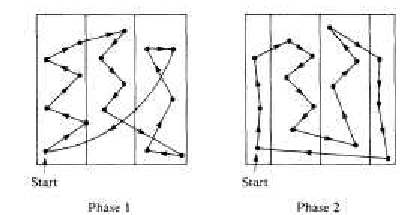
\includegraphics[width=1\linewidth]{images/fig-strip-alg-tsp.png}
\caption{The Strip Algorithm
                \label{fig-strip-alg-tsp}}
\end{figure}
\par
Step \hyperlink{step-1-3}{c} may need a bit more explanation. How do you travel up or down a strip? In most cases, the vertices in a strip will be vertically distributed so that the order in which they are visited is obvious. In some cases, however, the order might not be clear, as in the third strip in Phase I of
\hyperref[fig-strip-alg-tsp]{Figure~\ref{fig-strip-alg-tsp}}. Within a strip, the order in which you visit the points (if you are going up the strip) is determined thusly: \(\left(x_i,y_i\right)\)
precedes \(\left(x_j,y_j\right)\) if \(y_i <y_j\) or if \(y_i=y_j\) and \(x_i < x_j\) . In traveling down a strip, replace \(y_i < y_j\) with \(y_i >y_j\).%
\par
The selection of \(\left\lceil \sqrt{n/2}\right\rceil\) strips was made in a 1959 paper by Beardwood, Halton, and Hammersley. It balances the problems
that arise if the number of strips is too small or too large. If the square is divided into too few strips, some strips may be packed with vertices
so that visiting them would require excessive horizontal motion. If too many strips are used, excessive vertical motion tends to be the result. An update on what is known about this algorithm is contained in \hyperlink{biblio-sopowit-1983}{[1]}.%
\par
Since the construction of a circuit in the square consists of sorting the given points, it should come as no surprise that the strip algorithm requires
a time that is roughly a multiple of \(n \log  n\) time units when \(n\) points are to be visited.%
\par
The worst case that has been encountered with this algorithm is one in which the circuit obtained has a total distance of approximately \(\sqrt{2n}\)
(see Sopowit et al.).%
\typeout{************************************************}
\typeout{Subsection 1.5.3 Networks and the Maximum Flow Problem}
\typeout{************************************************}
\subsection[Networks and the Maximum Flow Problem]{Networks and the Maximum Flow Problem}\label{ss-networks-and-flows}
\index{Networks}\begin{definition}[Network]\label{def-network}
\index{Network} A network is a simple weighted directed graph that contains two distinguished vertices called the  source and the  sink with the properties that the indegree of the source and outdegree of the sink are both zero, and source is connected to sink.  The weight function on network is the capacity function, which as positive weights. %
\end{definition}
An example of a real situation that can be represented by a network is a city's water system. A reservoir would be the source, while a distribution
point in the city to all of the users would be the sink. The system of pumps and pipes that carries the water from source to sink makes up the remaining
network. We can assume that the water that passes through a pipe in one minute is controlled by a pump and the maximum rate is determined by the
size of the pipe and the strength of the pump. This maximum rate of flow through a pipe is called its capacity and is the information that the weight
function of a network contains.%
\begin{example}[A City Water System]\label{ex-city-water}
 Consider the system that is illustrated in \hyperref[fig-water-system]{Figure~\ref{fig-water-system}}. The numbers that appear next to each pipe indicate the capacity of
that pipe in thousands of gallons per minute. This map can be drawn in the form of a network, as in \hyperref[fig-water-network]{Figure~\ref{fig-water-network}}.
%
\leavevmode%
\begin{figure}
\centering
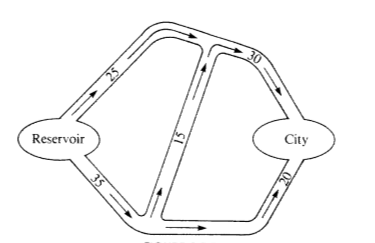
\includegraphics[width=1\linewidth]{images/fig-water-system.png}
\caption{City Water System
                \label{fig-water-system}}
\end{figure}
\leavevmode%
\begin{figure}
\centering
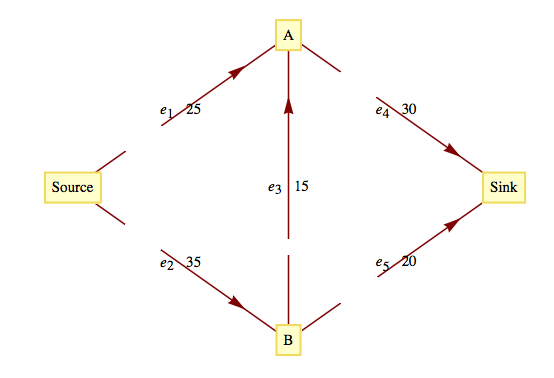
\includegraphics[width=1\linewidth]{images/fig-water-network.png}
\caption{Flow Diagrom for a City's Water Network
                \label{fig-water-network}}
\end{figure}
\par
Although the material passing through this network is water, networks can also represent the flow of other materials, such as automobiles, electricity, bits, telephone calls, or patients in a health system.%
\end{example}
\begin{problem}[The Maximum Flow Problem]\label{problem-maximal-flow}
The Maximum Flow Problem is derived from the objective of moving the maximum amount of water or other material from the source to the sink. To measure this amount, we define a flow as a function \(f: E \to \mathbb{R}\) such that (1) the flow of material through any edge is nonnegative and no larger
than its capacity: \(0 \leq  f(e) \leq  w(e)\), for all \(e\in  E\); and (2) for each vertex other than the source and sink, the total amount of material that is directed into a vertex is equal to the total amount that is directed out:

\begin{align}
\begin{array}{ccc}
 \sum_{(x,v)\in E} f(x,v)  & = & \sum_{(v,y)\in E} f(v,y) \\
 \textrm{Flow into } v & = & \textrm{ Flow out of } v \\
\end{array}\label{flow-rules}
\end{align}

The summation on the left of \hyperref[flow-rules]{(\ref{flow-rules})} represents the sum of the flows through each edge in \(E\) that has \(v\) as a terminal vertex.
The right-hand side indicates that you should add all of the flows through edges that initiate at \(v\).%
\end{problem}
\begin{theorem}[Flow out of Source equals Flow in Sink]\label{theorem-flow-inout}
 If \(f\) is a flow, then
\(\quad \quad\)\(\sum_{(\text{source},v)\in E} f(\text{source},v)\text{  }=\sum_{(v,\text{sink})\in E} f(v,\text{sink})\)  %
\end{theorem}
\begin{proof}\hypertarget{proof-4}{}
Subtract the right-hand side of \hyperref[flow-rules]{(\ref{flow-rules})} from the left-hand side. The result is: 
\[\text{Flow into } v - \text{ Flow out of } v = 0\]

 Now sum up these differences for each vertex in \(V' = V - \{\text{source}, \text{sink}\}\). The result is
\begin{gather}
\sum_{v\in V'}  \left(\sum_{(x,v)\in E} f(x,v)-\sum_{(v,y)\in E} f(v,y)\right)= 0\label{proof-step-9-5}
\end{gather}
%
\par
Now observe that if an edge connects two vertices in \(V'\), its flow appears as both a positive and a negative term in \hyperref[proof-step-9-5]{(\ref{proof-step-9-5})}. This means that the only positive terms that are not cancelled out are the flows into the sink. In addition, the only negative terms that remain are the flows out of the
source. Therefore,
\[\sum_{(v,\text{sink})\in E} f(v,\text{sink})-\sum_{(\text{source},v)\in E} f(\text{source},v) =0\]%
\end{proof}
\begin{definition}[The Value of a Flow]\label{def-value-of-flow}
\index{Value of a Flow}\label{notation-5}
The common value, as proven in \hyperref[theorem-flow-inout]{Theorem~\ref{theorem-flow-inout}}, flow into the sink and flow out of the source, is called the value of the flow. It is denoted by \(V(f)\). The value of a flow represents the amount of material that passes through the network with that flow.%
\end{definition}
\par
Since the Maximum Flow Problem consists of maximizing the amount of material that passes through a given network, it is equivalent to finding a flow with the largest possible value. Any such flow is called a \terminology{maximal flow}\index{Maximal flow}.%
\par
For the network in \hyperref[fig-water-network]{Figure~\ref{fig-water-network}}, one flow is \(f_1\), defined by \(f_1\left(e_1\right)=25\), \(f_1\left(e_2\right)=20\), \(f_1\left(e_3\right)=0\),
\(f_1\left(e_4\right)= 25\), and \(f_1\left(e_5\right)=20\). The value of \(f_1\), \(V\left(f_1\right)\), is 45. Since the total flow into the sink
can be no larger than 50 (\(w \left(e_4\right) + w \left(e_5\right) = 30 + 20\)), we can tell that \(f_1\) is not very far from the solution. Can
you improve on \(f_1\) at all? The sum of the capacities into the sink can't always be obtained by a flow. The same is true for the sum of the
capacities out of the source. In this case, the sum of the capacities out of the source is 60, which obviously can't be reached in this network.%
\par
A solution of the Maximum Flow Problem for this network is the maximal flow \(f_2\), where \(f_2\left(e_1\right)=25\), \(f_2\left(e_2\right)=25\),
\(f_2\left(e_3\right)=5\), \(f_2\left(e_4\right)= 30\), and \(f_2\left(e_5\right)=20\), with \(V\left(f_2\right) = 50\). This solution is not unique.
In fact, there is an infinite number of maximal flows for this problem.%
\par
There have been several algorithms developed to solve the Maximal Flow Problem. One of these is the Ford and Fulkerson Algorithm (FFA). The FFA consists of repeatedly finding paths in a network called flow augmenting paths until no improvement can be made in the flow that has been obtained.%
\begin{definition}[Flow Augmenting Path.]\label{def-flow-augmenting-path}
\index{Flow Augmenting Path}Given a flow \(f\) in a network \((V, E)\), a flow augmenting path with respect to \(f\) is a simple path from the
source to the sink using edges both in their forward and their reverse directions such that for each edge \(e\) in the path, \(w(e) - f(e) > 0\) if \(e\) is used in its forward direction and \(f(e) > 0\) if \(e\) is used in the reverse direction.
%
\end{definition}
\begin{example}[Augmenting City Water Flow]\label{example-water-augmenting}
For \(f_1\) in \hyperref[fig-water-network]{Figure~\ref{fig-water-network}}Example 9.5.6, a flow augmenting path would be\(\left(e_2 , e_3 , e_4 \right)\) since
\(w\left(e_2\right)-f_1\left(e_2\right)= 15\), \(w\left(e_3\right)-f_1\left(e_3\right)=5\), and \(w\left(e_4\right)-f_1\left(e_4\right)=5\).%
\par
These positive differences represent unused capacities, and the smallest value represents the amount of flow that can be added to each edge in the path. Note that by adding 5 to each edge in our path, we obtain \(f_2\), which is maximal. If an edge with a positive flow is used in its reverse direction, it is contributing a movement of material that is counterproductive to the objective of maximizing flow. This is why the
algorithm directs us to decrease the flow through that edge.%
\end{example}
\begin{algorithm}[The Ford and Fulkerson Algorithm]\label{alg-ford-fulkerson}
\leavevmode%
\begin{enumerate}[label=\arabic*]
\item\hypertarget{li-80}{} Define the flow function \(f_0\) by \(f_0(e)=0\) for each edge \(e \in  E\).%
\item\hypertarget{li-81}{}i = 0.%
\item\hypertarget{li-82}{}Repeat:%
\par
%
\begin{enumerate}[label=\alph*]
\item\hypertarget{li-83}{}If possible, find a flow augmenting path with respect to \(f_i\).%
\item\hypertarget{li-84}{}If a flow augmenting path exists, then:%
\par
%
\begin{enumerate}[label=\roman*]
\item\hypertarget{li-85}{}Determine
		   \[d = \min  \left\{\left\{\left.w(e) - f_i(e) \right| e \text{is used in the forward direction}\right\},\left\{\left.f_i(e) \right| e \text{is used in the reverse direction}\right\}\right\}\]%
\item\hypertarget{li-86}{}Define \(f_{i+1}\) by \[\begin{array}{cc}
 f_{i+1}(e) = f_i(e) &  \text{if } e \text{ is not part of the flow augmenting path} \\
 f_{i+1}(e)=f_i(e)+d & \text{if } e \text{ is used in the forward direction} \\
 f_{i+1}(e)=f_i(e)-d & \text{if } e \text{ is used in the reverse direction} \\
\end{array}\]%
\item\hypertarget{li-87}{} \(i = i + 1\)%
\end{enumerate}
%
\end{enumerate}
%
\par
 until no flow augmenting path exists.%
\item\hypertarget{li-88}{}Terminate with a maximal flow \(f_i\)%
\end{enumerate}
%
\end{algorithm}
\begin{listwrapper}[Notes on the Ford and Fulkerson Algorithm]\label{list-8}
\leavevmode%
\begin{enumerate}[label=\arabic*]
\item\hypertarget{li-89}{} It should be clear that every flow augmenting path leads to a flow of increased value and that none of the capacities of the network can be violated.%
\item\hypertarget{li-90}{} The depth-first search should be used to find flow augmenting paths since it is far more efficient than the breadth-first search in this situation. The depth-first search differs from the breadth-first algorithm  in that you sequentially visit vertices
until you reach a ``dead end'' and then backtrack.%
\item\hypertarget{li-91}{} There have been networks discovered for which the FFA does not terminate in a finite number of steps. These examples all have irrational capacities. It has been proven that if all capacities are positive integers, the FFA terminates in a finite number of steps. See Ford and Fulkerson, Even, or Berge for details.%
\item\hypertarget{li-92}{} When you use the FFA to solve the Maximum Flow Problem by hand it is convenient to label each edge of the network with the fraction \(\frac{f_i(e)}{w(e)}\).%
\end{enumerate}
\end{listwrapper}
\begin{algorithm}[Depth-First Search for a Flow Augmenting Path]\label{alg-depth-first-search}
 This is a  depth-first search for the Sink Initiating at the Source. Let \(E'\) be the set of directed edges that can be used in producing a flow augmenting path. Add to the network a vertex called  start and the edge \((\text{start}, \text{source}).\)%
\par
\leavevmode%
\begin{enumerate}[label=\arabic*]
\item\hypertarget{li-93}{}\(S = \)vertex set of the network.%
\item\hypertarget{li-94}{}\(p= \)start%
\item\hypertarget{li-95}{}\(p = \)source \(\quad \quad\)  Move \(p\) along the edge \((start, source)\) %
\item\hypertarget{li-96}{}while \(p\) is not equal to  start or  sink:%
\par
%
\begin{enumerate}[label=\alph*]
\item\hypertarget{li-97}{}if an edge in \(E'\) exists that takes you from \(p\) to another vertex in \(S\):
\begin{equation*}\quad \text{then set } p \text{ to be that next vertex and delete the edge from } E'\end{equation*}
\begin{equation*}\quad \text{else reassign }p \text{ to be the vertex that }p\text{ was reached from (i.e., backtrack)}\end{equation*}%
\end{enumerate}
%
\item\hypertarget{li-98}{}\(\text{if } p = \text{start:}\) 
		\begin{equation*}\text{ then no flow augmenting path exists.}\end{equation*}
		\begin{equation*}\text{ else }p = \text{sink and you have found a flow augmenting path.}\end{equation*}
%
\end{enumerate}
%
\end{algorithm}
\begin{example}[A flow augmenting path going against the flow]\label{ex-fap-1}
 Consider the network in \hyperref[fig-flow-example-before]{Figure~\ref{fig-flow-example-before}}, where the current flow, \(f\), is indicated by a labeling of the edges. %
\leavevmode%
\begin{figure}
\centering
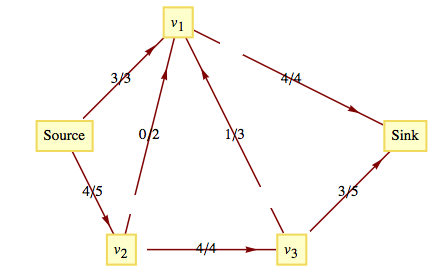
\includegraphics[width=1\linewidth]{images/fig-flow-example-before.png}
\caption{Current Flow
                \label{fig-flow-example-before}}
\end{figure}
\par
The path
\(\left(S\text{ource}, v_2 , v_1,v_3 , S\text{ink}\right)\) is a flow augmenting path that allows us to increase the flow by one
unit. Note that \(\left(v_1,v_3\right)\) is used in the reverse direction, which is allowed because \(f\left(v_1,v_3\right)>0\). The value of
the new flow that we obtain is 8. This flow must be maximal since the capacities out of the source add up to 8. This maximal flow is defined by \hyperref[fig-updated-flow]{Figure~\ref{fig-updated-flow}}.%
\leavevmode%
\begin{figure}
\centering
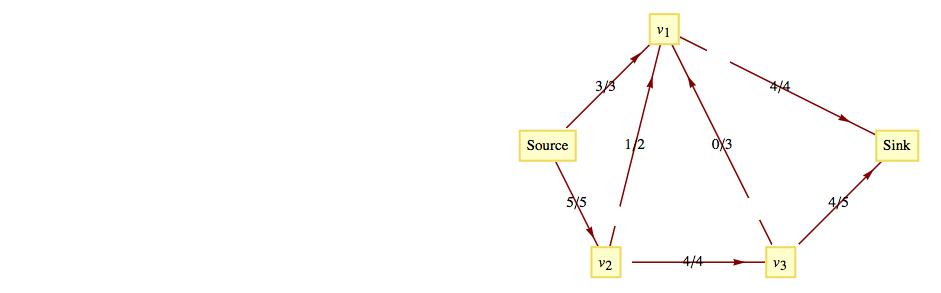
\includegraphics[width=1\linewidth]{images/fig-updated-flow.png}
\caption{Updated Flow
                \label{fig-updated-flow}}
\end{figure}
\end{example}
\typeout{************************************************}
\typeout{Subsection 1.5.4 Other Graph Optimization Problems}
\typeout{************************************************}
\subsection[Other Graph Optimization Problems]{Other Graph Optimization Problems}\label{ss-other-optimization}
\leavevmode%
\begin{enumerate}[label=\arabic*]
\item\hypertarget{li-99}{}  The Minimum Spanning Tree Problem: Given a weighted graph, \((V, E, w)\), find a subset \(\text{E'}\) of \(E\) with
the properties that \((V, E')\) is connected and the sum of the weights of edges in \(E'\) are as small as possible. We will discuss this problem in Chapter 10.%
\item\hypertarget{li-100}{}  The Minimum Matching Problem: Given an undirected weighted graph, \((K, E, w)\), with an even number of vertices, pair up the vertices
so that each pair is connected by an edge and the sum of these edges is as small as possible. A unit square version of this problem has been studied extensively. See \hyperlink{biblio-sopowit-1983}{[1]} for details on what is known about this version of the problem. %
\item\hypertarget{li-101}{}  The Graph Center Problem: Given a connected, undirected, weighted graph, find a vertex (the center) in the graph with the property
that the distance from the center to every other vertex is as small as possible. ``As small as possible'' could be interpreted either as minimizing the sum of the distances to each vertex or as minimizing the maximum distance from the center to a vertex.
%
\end{enumerate}
%
\typeout{************************************************}
\typeout{Exercises 1.5.5 Exercises for Section 9.5}
\typeout{************************************************}
\subsection[Exercises for Section 9.5]{Exercises for Section 9.5}\label{exercises-9-5}
\hypertarget{exercisegroup-7}{}\typeout{************************************************}
\typeout{Introduction  }
\typeout{************************************************}
A Exercises%
\begin{exercisegroup}
\item[1.]\hypertarget{exercise-31}{} Find the closest neighbor circuit through the six capitals of New England starting at Boston. If you start at a different city, will you get a different circuit?%
\par\smallskip
\par\smallskip
\noindent\textbf{Answer.}\hypertarget{answer-11}{}\quad
 The circuit would be Boston, Providence, Hartford, Concord, Montpelier, Augusta, Boston. It does matter where you start. If you start in Concord,
for example, your mileage will be higher.%
\item[2.]\hypertarget{exercise-32}{} Is Theorem 9.5.1 sharp for \(n = 3\)? For \(n = 4\)?%
\par\smallskip
\item[3.]\hypertarget{exercise-33}{} Given the following sets of points in the unit square, find the shortest circuit that visits all the points and find the circuit that is obtained
with the strip algorithm.%
\par
\leavevmode%
\begin{enumerate}[label=\alph*]
\item\hypertarget{li-102}{} \(\{(0.1k, 0.1k) : k = 0, 1, 2, . . . , 10\}\)%
\item\hypertarget{li-103}{} \(\{(0.1, 0.3), (0.3, 0.8), (0.5, 0.3), (0.7, 0.9), (0.9, 0.1)\}\)%
\item\hypertarget{li-104}{} \(\{(0.0, 0.5), (0.5, 0.0), (0.5, 1.0), (1.0, 0.5)\}\)%
\item\hypertarget{li-105}{} \(\{(0, 0), (0.2, 0.6), (0.4, 0.1), (0.6, 0.8), (0.7, 0.5)\}\)%
\end{enumerate}
%
\par\smallskip
\par\smallskip
\noindent\textbf{Answer.}\hypertarget{answer-12}{}\quad
\leavevmode%
\begin{enumerate}[label=\alph*]
\item\hypertarget{li-106}{} Optimal cost \(=2\sqrt{2}\).
Phase 1 cost \(=2.4\sqrt{2}\).
Phase 2 cost \(=2.6\sqrt{2}\).
%
\item\hypertarget{li-107}{} Optimal cost \(=2.60.\) 
Phase 1 cost \(=3.00\). 
Phase 2 cost \(2\sqrt{2}\).
%
\item\hypertarget{li-108}{}  \(A=(0.0, 0.5), B=(0.5, 0.0), C=(0.5, 1.0), D=(1.0, 0.5)\)
here are 4 points; so we will divide the unit square into two strips. 
Optimal Path: \((B,A,C,D)\quad \quad \text{Distance } =2\sqrt{2}\) 
Phase I Path: \((B,A,C,D)\quad \quad \text{Distance }=2\sqrt{2}\) 
Phase II Path: \((A,C,B,D)\quad \quad \text{Distance }=2+\sqrt{2}\)
%
\item\hypertarget{li-109}{} \(A=(0,0), B=(0.2,0.6), C=(0.4,0.1), D=(0.6,0.8), E=(0.7,0.5)\)
There are 5 points; so we will divide the unit square into three strips.
Optimal Path: \((A,B,D,E,C)\quad \quad \text{Distance }=2.31\)
Phase I Path: \((A,C,B,C,E)\quad \quad \text{Distance } = 2.57
Phase II Path: \((A,B,D,E,C)\quad \quad \text{Distance }=2.31\)
%
\end{enumerate}
%
\item[4.]\hypertarget{exercise-34}{} For \(n = 4, 5, \text{and } 6\), locate \(n\) points in the unit square for which the strip algorithm works poorly.%
\par\smallskip
\item[5.]\hypertarget{exercise-35}{} Consider the network whose maximum capacities are shown on the following graph.%
\leavevmode%
\begin{figure}
\centering
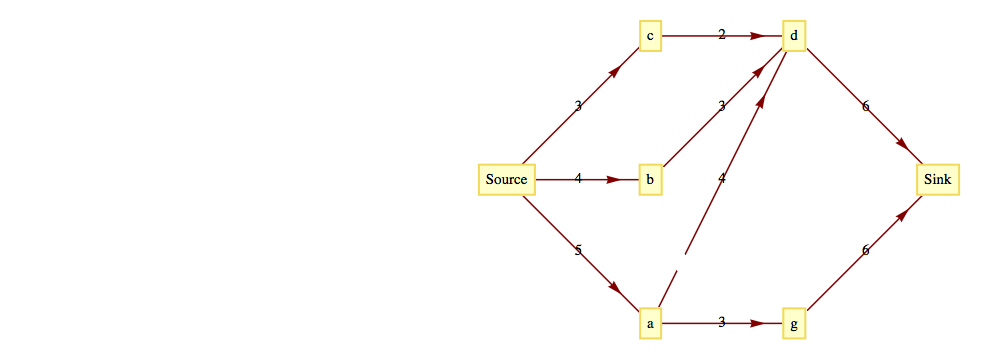
\includegraphics[width=1\linewidth]{images/fig-exercise-9-5-5.png}
\end{figure}
\par
\leavevmode%
\begin{enumerate}[label=\alph*]
\item\hypertarget{li-110}{} A function \(f\) is partially defined on the edges of this network by:
\(\quad \quad\)\(f(\text{Source}, c) = f(\text{Source}, b) =f(\text{Source}, a) = 2\), and \(f(a, d) = 1\). 
 Define \(f\) on the rest of the other edges so that \(f\) is a flow. What is the value of  \(f\) ?%
\item\hypertarget{li-111}{} Find a flow augmenting path with respect to \(f\) for this network. What is the value of the augmented flow?%
\item\hypertarget{li-112}{} Is the augmented flow a maximum flow? Explain.%
\end{enumerate}
%
\par\smallskip
\par\smallskip
\noindent\textbf{Answer.}\hypertarget{answer-13}{}\quad
\leavevmode%
\begin{enumerate}[label=\alph*]
\item\hypertarget{li-113}{} \(f(c,d)=2, f(b,d)=2, f(d,k)=5, f(a,g)=1, \text{and} f(g,k)=1\).
%
\item\hypertarget{li-114}{}  There are three possible flow-augmenting paths.

\(s,b,d,k\) with flow increase of 1.
\(s,a,d,k\) with flow increase of 1, and
\(s,a,g,k\) with flow increase of 2.
%
\item\hypertarget{li-115}{}  The new flow is never maximal, since another flow-augmenting path will always exist. For example, if \(s,b,d,k\) is used above, the new flow
can be augmented by 2 units with \(s,a,g,k\).
%
\end{enumerate}
%
\item[6.]\hypertarget{exercise-36}{} Given the following network with capacity function \(c\) and flow function \(f\), find a maximal flow function. The labels on thevedges of the network are of the form \(f(e)/c(e)\), where \(c(e)\) is the capacity of edge \(e\) and \(f(e)\) is the used capacity for flow
\(f\).%
\leavevmode%
\begin{figure}
\centering
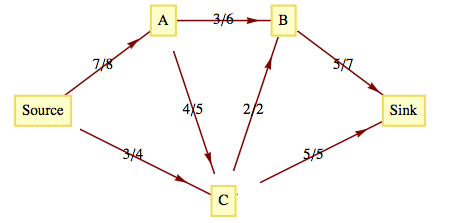
\includegraphics[width=1\linewidth]{images/fig-exercise-9-5-6.png}
\end{figure}
\par\smallskip
\item[7.]\hypertarget{exercise-37}{} Find maximal flows for the following networks.%
% group protects changes to lengths, releases boxes (?)
{% begin: group for a single side-by-side
% set panel max height to practical minimum, created in preamble
\setlength{\panelmax}{0pt}
\newsavebox{\panelboxAIimage}
\savebox{\panelboxAIimage}{
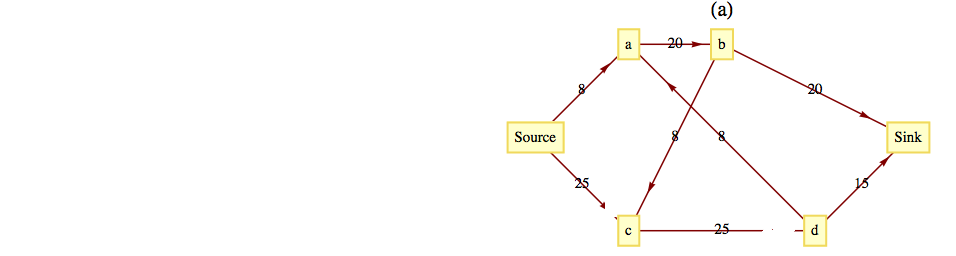
\includegraphics[width=0.5\linewidth]{images/fig-exercise-9-5-7a.png}
}
\newlength{\phAIimage}\setlength{\phAIimage}{\ht\panelboxAIimage+\dp\panelboxAIimage}
\settototalheight{\phAIimage}{\usebox{\panelboxAIimage}}
\setlength{\panelmax}{\maxof{\panelmax}{\phAIimage}}
\newsavebox{\panelboxAJimage}
\savebox{\panelboxAJimage}{
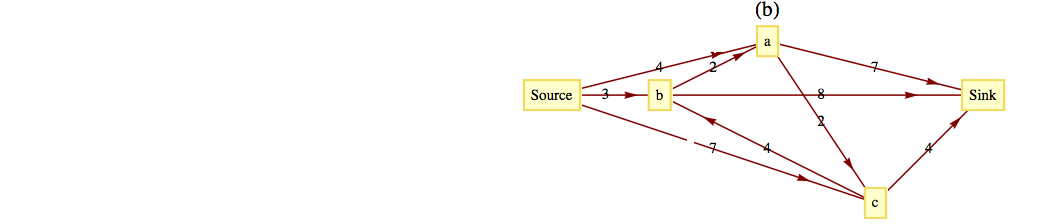
\includegraphics[width=0.5\linewidth]{images/fig-exercise-9-5-7b.png}
}
\newlength{\phAJimage}\setlength{\phAJimage}{\ht\panelboxAJimage+\dp\panelboxAJimage}
\settototalheight{\phAJimage}{\usebox{\panelboxAJimage}}
\setlength{\panelmax}{\maxof{\panelmax}{\phAJimage}}
\leavevmode%
% begin: side-by-side as figure/tabular
% \tabcolsep change local to group
\setlength{\tabcolsep}{0\textwidth}
% @{} suppress \tabcolsep at extremes, so margins behave as intended
\begin{figure}
\begin{tabular}{@{}*{2}{c}@{}}
\begin{minipage}[c][\panelmax][t]{0.5\textwidth}\usebox{\panelboxAIimage}\end{minipage}&
\begin{minipage}[c][\panelmax][t]{0.5\textwidth}\usebox{\panelboxAJimage}\end{minipage}\end{tabular}
\end{figure}
% end: side-by-side as tabular/figure
}% end: group for a single side-by-side
\leavevmode%
\begin{figure}
\centering
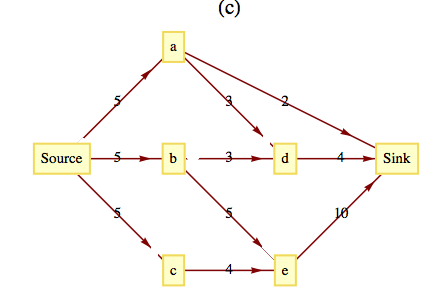
\includegraphics[width=1\linewidth]{images/fig-exercise-9-5-7c.png}
\end{figure}
\par\smallskip
\par\smallskip
\noindent\textbf{Answer.}\hypertarget{answer-14}{}\quad
\leavevmode%
\begin{enumerate}[label=\alph*]
\item\hypertarget{li-116}{} Value of maximal flow \(=31\).%
\item\hypertarget{li-117}{} Value of maximal flow \(=14\).%
\item\hypertarget{li-118}{} Value of maximal flow \(=14\). See \hyperref[table-solution-9-5-7]{Table~} for one way to got this flow.%
\end{enumerate}
%
\leavevmode%
\begin{table}
\centering
\begin{tabular}{ccc}\hrulethick
Step&Flow-augmenting path&Flow added\tabularnewline[0pt]
1&\(\text{Source},A,\text{Sink}\)&2\tabularnewline[0pt]
2&\(\text{Source}, C,B, \text{Sink}\)&3\tabularnewline[0pt]
3&\(\text{Source},E,D, \text{Sink}\)&4\tabularnewline[0pt]
4&\(\text{Source},A,B,\text{Sink}\)&1\tabularnewline[0pt]
5&\(\text{Source},C,D, \text{Sink}\)&2\tabularnewline[0pt]
6&\(\text{Source},A,B,C,D, \text{Sink}\)&2
\end{tabular}
\end{table}
\end{exercisegroup}
\par\smallskip\noindent
\hypertarget{exercisegroup-8}{}\typeout{************************************************}
\typeout{Introduction  }
\typeout{************************************************}
B Exercises%
\begin{exercisegroup}
\item[8.]\hypertarget{exercise-38}{}\leavevmode%
\begin{enumerate}[label=\alph*]
\item\hypertarget{li-119}{} [Easy] Find two maximal flows for the network in Figure 9.5.6 other than the one found in the text.%
\item\hypertarget{li-120}{}  [Harder] Describe the set of all maximal flows for the same network.%
\item\hypertarget{li-121}{}  [Hardest] Prove that if a network has two maximal flows, then it has an infinite number of maximal flows.%
\end{enumerate}
%
\par\smallskip
\item[9.]\hypertarget{exercise-39}{}Discuss reasons that the closest neighbor algorithm is not used in the unit square version of the Traveling Salesman Problem.%
\par\smallskip
\par\smallskip
\noindent\textbf{Hint.}\hypertarget{hint-2}{}\quad
Count the number of comparisons of distances that must be done.%
\par\smallskip
\noindent\textbf{Answer.}\hypertarget{answer-15}{}\quad
 To locate the closest neighbor among the list of \(k\) other points on the unit square requires a time proportional to \(k\). Therefore
the time required for the closest-neighbor algorithm with \(n\) points is proportional to \((n-1)+(n-2)+\cdots +2+1\), which is proportional
to \(n^2\). Since the strip algorithm takes a time proportional to \(n(\log  n)\), it is much faster for large values of \(n\).
%
\end{exercisegroup}
\par\smallskip\noindent
\hypertarget{exercisegroup-9}{}\typeout{************************************************}
\typeout{Introduction  }
\typeout{************************************************}
C Exercises%
\begin{exercisegroup}
\item[10.]\hypertarget{exercise-40}{} Explore the possibility of solving the Traveling Salesman Problem in the ``unit box'': \([0,1]^3\).%
\par\smallskip
\item[11.]\hypertarget{exercise-41}{} Devise a ``closest neighbor'' algorithm for matching points in the unit square.
%
\par\smallskip
\end{exercisegroup}
\par\smallskip\noindent
\typeout{************************************************}
\typeout{Section 1.6 Planarity and Colorings}
\typeout{************************************************}
\section[Planarity and Colorings]{Planarity and Colorings}\label{s-planarity-and-colorings}
\typeout{************************************************}
\typeout{Introduction  }
\typeout{************************************************}
The topics in this section are related to how graphs are drawn.%
\par
Planarity: Can a given graph be drawn in a plane so that no edges intersect? Certainly, it is natural to avoid intersections, but up to now we haven't gone out of our way to do so.%
\par
Colorings: Suppose that each vertex in an undirected graph is to be colored so that no two vertices that are connected by an edge have the
same color. How many colors are needed? This question is motivated by the problem of drawing a map so that no two bordering countries are colored
the same. A similar question can be asked for coloring edges.%
\typeout{************************************************}
\typeout{Subsection 1.6.1 Planar Graphs}
\typeout{************************************************}
\subsection[Planar Graphs]{Planar Graphs}\label{ss-planarity}
\begin{definition}[Planar Graph/Plane Graph]\label{def-planar-graph}
\index{Planar Graph}\index{Plane Graph}\label{notation-6}
A graph is planar if it can be drawn in a plane so that no edges cross. If a
graph is drawn so that no edges intersect, it is a plane graph, and such a drawing is a planar embedding of the graph.%
\end{definition}
\begin{example}[A Planar Graph]\label{ex-planar-graph}
The graph in \hyperref[fig-planar-plane]{Figure~\ref{fig-planar-plane}}(a) is planar but not a plane graph. The same graph is drawn as a plane graph in \hyperref[fig-planar-plane]{Figure~\ref{fig-planar-plane}}(b).%
\leavevmode%
\begin{figure}
\centering
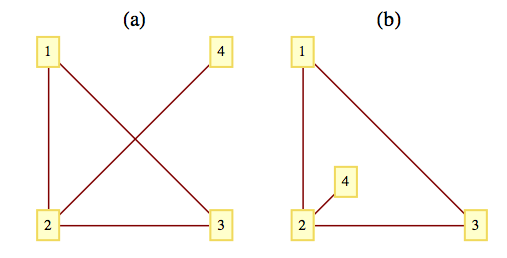
\includegraphics[width=1\linewidth]{images/fig-planar-plane.png}
\caption{A Planar Graph
                \label{fig-planar-plane}}
\end{figure}
\end{example}
\leavevmode%
\begin{enumerate}[label=\alph*]
\item\hypertarget{li-122}{} In discussing planarity, we need only consider simple undirected graphs with no self-loops. All other graphs can be treated as such since
all of the edges that relate any two vertices can be considered as one ``package'' that clearly can be drawn in a plane.%
\item\hypertarget{li-123}{} Can you think of a graph that is not planar? How would you prove that it isn't planar? Proving the nonexistence of something is usually more
difficult than proving its existence. This case is no exception. Intuitively, we would expect that sparse graphs would be planar and dense graphs
would be nonplanar. Theorem 9.6.2 will verify that dense graphs are indeed nonplanar.%
\item\hypertarget{li-124}{} The topic of planarity is a result of trying to restrict a graph to two dimensions. Is there an analogous topic for three dimensions? What
graphs can be drawn in one dimension?%
\end{enumerate}
%
\begin{observation}[Graphs in other dimensions]\label{observation-2}
 If a graph has only a finite number of vertices, it can always be drawn in three dimensions. This is not true for all graphs with
an infinite number of vertices. The only ``one-dimensional'' graphs are the ones that consist of a finite number of chains, as in Figure 9.6.2,
with one or more vertices in each chain.%
\leavevmode%
\begin{figure}
\centering
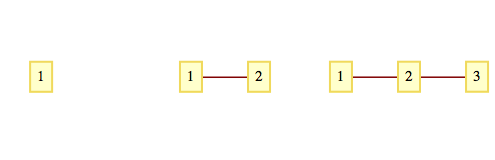
\includegraphics[width=1\linewidth]{images/fig-chains.png}
\caption{Chains - one dimensional graphs
                \label{fig-chains}}
\end{figure}
\end{observation}
\par
\index{Three Utilities Puzzle}A discussion of planarity is not complete without mentioning the famous Three Utilities Puzzle. The object
of the puzzle is to supply three houses, A, B, and C, with the three utilities, gas, electric, and water. The constraint that makes this puzzle impossible
to solve is that no utility lines may intersect i. e., a planar embedding of the graph in \hyperref[fig-utilities-puzzle]{Figure~\ref{fig-utilities-puzzle}}, which is commonly denoted \(K_{3,3}\). This graph is one of two fundamental nonplanar graphs. The Kuratowski Reduction Theorem states that if a graph is nonplanar then ``contains'' either a \(K_{3,3}\) or a \(K_5\).  Containment is in the sense that if you start with a nonplanar graph you can always perform a sequence of
edge deletions and contractions (shrinking an edge so that the two vertices connecting it coincide) to produce one of the two graphs.%
\leavevmode%
\begin{figure}
\centering
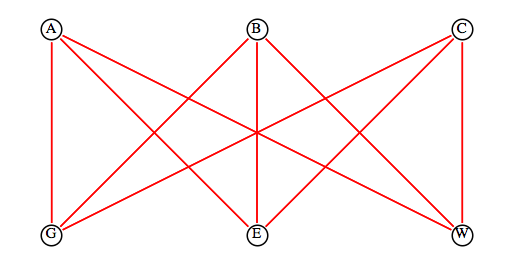
\includegraphics[width=1\linewidth]{images/fig-utilities-puzzle.png}
\caption{The Three Utilities Puzzle
                \label{fig-utilities-puzzle}}
\end{figure}
\par
A planar graph divides the plane into one or more regions. Two points on the plane lie in the same region if you can draw a curve connecting the
two points that does not pass through an edge. One of these regions will be of infinite area. Each point on the plane is either a vertex, a point on an edge, or a point in a region. A remarkable fact about the geography of planar graphs is the following theorem that is attributed to Euler.%
\begin{task}[]\label{task-1}
Experiment: Jot down a graph right now and count the number of vertices, regions, and edges that you have. If \(v + r - e\) is not 2, then your graph
is either nonplanar or not connected.%
\end{task}
\begin{theorem}[Euler's Formula]\label{theorem-euler-formula}
\index{Euler's Formula}If \(G = (V, E)\) is a connected planar graph with \(r\) regions, \(v\) vertices and \(e\) edges, then
\begin{gather}
v + r - e = 2\label{euler-formula}
\end{gather}%
\end{theorem}
\begin{proof}\hypertarget{proof-5}{}
We prove Euler's Formula by Induction on \(e\), for \(e \geq  0\).%
\par
Basis: If \(e = 0\), then \(G\) must be a graph with one vertex, \(v = 1\); and there is one infinite region,\(\text{  }r = 1\). Therefore, \(v + r-e= 1 + 1-0 = 2\), and the basis is true.%
\par
Induction: Suppose that \(G\) has \(k\) edges, \(k \geq  1\), and that all connected planar graphs with less than \(k\) edges satisfy
9.6a. Select any edge that is part of the boundary of the infinite region and call it \(e_1\). Let \(G'\) be the graph obtained from \(G\)
by deleting \(e_1\). Figure 9.6.4 illustrates the two different possibilities we need to consider: either \(G'\) is connected or it has two
connected components, \(G_1\) and \(G_2\).%
\leavevmode%
\begin{figure}
\centering
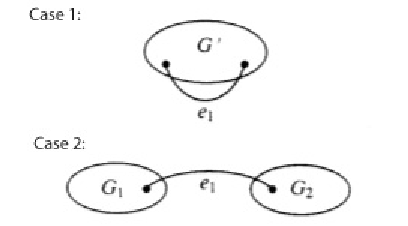
\includegraphics[width=1\linewidth]{images/fig-euler-proof-scheme.png}
\caption{Two cases in the proof of Euler's Formula
                \label{fig-euler-proof-scheme}}
\end{figure}
\par
If \(G'\) is connected, the induction hypothesis can be applied to it. If \(G'\) has \(v'\) vertices, \(r'\) edges and \(e'\) edges, then \(v'+r'-e'=2\) and in terms of the corresponding numbers for \(G\), 

   \[\begin{array}{ll}
 v'=v & \textrm{ No vertices were removed to form } G' \\
 r'=r-1 & \textrm{ One region of } G \textrm{ was merged with the infinite region when } e_1 \textrm{ was removed}
\\
 e' = k-1 & \textrm{We assumed that} G \textrm{ had } k \textrm{ edges.} \\
\end{array}\]%
\par
For the case where \(G'\) is connected, 

\begin{equation*}\begin{split}
v+ r -e &= v+r-k\\
	&= v' + (r'+1) -(e'+1)\\
	& = v' + r'-e'\\
	& =2
\end{split}
\end{equation*}

If \(G'\) is not connected, it must consist of two connected components, \(G_1\)  and \(G_2\) since
we started with a connected graph, \(G\). We can apply the induction hypothesis to each of the two components to complete the proof. 
We leave it to the students to do this, with the reminder that in counting regions, \(G_1\)  and \(G_2\)  will share the same
infinite region.%
\end{proof}
\begin{theorem}[A Bound on Edges of a Planar Graph]\label{theorem-edge-bound}
If \(G = (V, E)\) is a connected planar graph with \(v\) vertices, \(v\geq 3\), and \(e\) edges, then
\begin{gather}
e \leq  3v - 6\label{edge-bound}
\end{gather}
%
\end{theorem}
\begin{proof}\hypertarget{proof-6}{}
(Outline of a Proof)%
\par
\leavevmode%
\begin{enumerate}[label=\alph*]
\item\hypertarget{li-125}{} Let \(r\) be the number of regions in \(G\). For each region, count the number of edges that comprise its border. The sum of these counts must be at least  3r. Recall that we are working with simple graphs here, so a region made by two edges connecting the same two
vertices is not possible.%
\item\hypertarget{li-126}{} Based on (a), infer that the number of edges in \(G\) must be at least \(\frac{3 r}{2}\).%
\item\hypertarget{li-127}{} \(e\geq \frac{3r}{2}\text{   }\Rightarrow \text{      }r\leq \frac{2e}{3}\)%
\item\hypertarget{li-128}{}Substitute \(\frac{2e}{3}\) for \(r\) in Euler's Formula to obtain an inequality that is equivalent to  \hyperref[edge-bound]{(\ref{edge-bound})}%
\end{enumerate}
%
\end{proof}
\begin{remark}[]\label{remark-1}
One implication of \hyperref[edge-bound]{(\ref{edge-bound})} is that the number of edges in a connected planar graph will never be larger than three times its
number of vertices (as long as it has at least three vertices). Since the maximum number of edges in a graph with \(v\) vertices is a quadratic function of \(v\), as \(v\) increases, planar graphs are more and more sparse.%
\end{remark}
\par
The following theorem will be useful as we turn to graph coloring.%
\begin{theorem}[A Vertex of Degree Five]\label{theorem-degree-5}
If \(G\) is a connected planar graph, then it has a vertex with degree 5 or less.%
\end{theorem}
\begin{proof}\hypertarget{proof-7}{}
(by contradiction): We can assume that \(G\) has at least seven vertices, for otherwise the degree of any vertex is at most 5.
Suppose that \(G\) is a connected planar graph and each vertex has a degree of 6 or more. Then, since each edge contributes to the degree
of two vertices, \(e\geq \frac{6v}{2}=3v\). However,\hyperref[theorem-edge-bound]{Theorem~\ref{theorem-edge-bound}}  states that the \(e\leq 3v-6 < 3v\), which is a contradiction.%
\end{proof}
\typeout{************************************************}
\typeout{Subsection 1.6.2 Graph Coloring}
\typeout{************************************************}
\subsection[Graph Coloring]{Graph Coloring}\label{ss-graph-coloring}
\leavevmode%
\begin{figure}
\centering
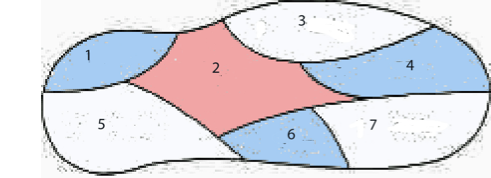
\includegraphics[width=1\linewidth]{images/fig-euler-island.png}
\caption{A 3-coloring of Euler Island
                \label{fig-euler-island}}
\end{figure}
The map of Euler Island in \hyperref[fig-euler-island]{Figure~\ref{fig-euler-island}} shows that there are seven towns on the island. Suppose that a cartographer must produce a colored map in
which no two towns that share a boundary have the same color. To keep costs down, she wants to minimize the number of different colors that appear
on the map. How many colors are sufficient? For Euler Island, the answer is three. This problem motivates a more general problem.%
\begin{definition}[Graph Coloring]\label{def-graph-coloring}
\index{Graph Coloring}\index{Chromatic Number}\label{notation-7}
Given an undirected graph \(G = (V, E)\), find a ``coloring function'' \(f\) from \(V\) into a
set of colors \(H\) such that \(\left(v_i,v_j\right)\in E \Rightarrow  f\left(v_i\right)\neq f\left(v_j\right)\) and \(H\) has the smallest
possible cardinality. The cardinality of \(H\) is called the  chromatic number of G, \(\chi(G)\).%
\end{definition}
\par
\leavevmode%
\begin{itemize}[label=\textbullet]
\item{} A coloring function onto an \(n\) element set is called an \(n\)-coloring.%
\item{} In terms of this general problem, the chromatic number of the graph of Euler Island is three. To see that no more than three colors are needed,
we need only display a 3-coloring: \(f(1) = f(4) = f(6) = \text{blue}\), \(f(2) = \text{red}\), and \(f(3) = f(5) = f(7) = \text{white}\). This coloring
is not unique. The next smallest set of colors would be of two colors, and you should be able to convince yourself that no 2-coloring exists for
this graph.
%
\end{itemize}
%
\par
In the mid-nineteenth century, it became clear that the typical planar graph had a chromatic number of no more than 4. At that point, mathematicians
attacked the Four-Color Conjecture, which is that if \(G\) is any planar graph, then its chromatic number is no more than 4. Although the conjecture
is quite easy to state, it took over 100 years, until 1976, to prove the conjecture in the affirmative.%
\begin{theorem}[The Four-Color Theorem.]\label{theorem-four-color-theorem}
\index{Four-Color Theorem.}If \(G\) is a planar graph, then \(\chi (G)\leq 4\).%
\end{theorem}
\par
A proof of the Four-Color Theorem is beyond the scope of this text, but we can prove a theorem that is only 25 percent inferior.%
\begin{theorem}[The Five-Color Theorem]\label{theorem-five-color-theorem}
\index{Five-Color Theorem}If \(G\) is a planar graph, then \(\chi (G)\leq 5\).%
\end{theorem}
\begin{proof}\hypertarget{proof-8}{}
The number 5 is not a sharp upper bound for \(\chi(G)\) because of the Four-Color Theorem.%
\par
This is a proof by Induction on the Number of Vertices in the Graph.%
\par
Basis: Clearly, a graph with one vertex has a chromatic number of 1.%
\par
Induction: Assume that all planar graphs with \(n - 1\) vertices have a chromatic number of 5 or less. Let \(G\) be a planar graph. By Theorem
9.6.2, there exists a vertex \(v\) with \(\deg  v \leq 5\). Let \(G - v\) be the planar graph obtained by deleting \(v\) and all edges
that connect \(v\) to other vertices in \(G\). By the induction hypothesis, \(G - v\) has a 5-coloring. Assume that the colors used
are red, white, blue, green, and yellow. %
\par
If \(\deg  v < 5\), then we can produce a 5-coloring of \(G\) by selecting a color that is not used in coloring the vertices that are connected
to \(v\) with an edge in \(G\).%
\par
If \(\deg  v = 5\), then we can use the same approach if the five vertices that are adjacent to \(v\) are not all colored differently. We are
now left with the possibility that \(v_1\), \(v_2\), \(v_3\), \(v_4\), and \(v_5\) are all connected to \(v\) by an edge and they are all colored
differently. Assume that they are colored red, white blue, yellow, and green, respectively, as in \hyperref[fig-five-coloring-proof]{Figure~}. %
\leavevmode%
\begin{figure}
\centering
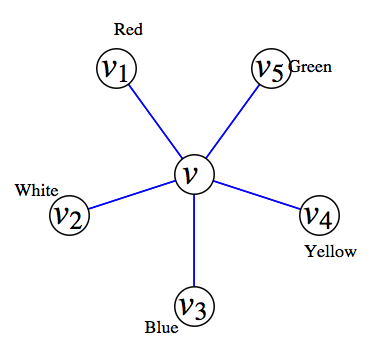
\includegraphics[width=1\linewidth]{images/fig-five-coloring-proof.png}
\end{figure}
\par
Starting at \(v_1\) in \(G-v\), suppose we try to construct a path \(v_3\) that passes through only red and blue vertices.  This can either be
accomplished or it can't be accomplished. If it can't be done, consider all paths that start at \(v_1\), and go through only red and blue vertices.
If we exchange the colors of the vertices in these paths, including \(v_1\) we still have a 5-coloring of \(G - v\). Since \(v_1\) is now blue, we
can color the central vertex, \(v\), red.%
\par
Finally, suppose that \(v_1\) is connected to \(v_3\) using only red and blue vertices. Then a path from \(v_{1 }\)to \(v_3\) by using red and blue
vertices followed by the edges \(\left(v_3,v\right)\) and \(\left(v,v_1\right)\) completes a circuit that either encloses \(v_2\) or encloses \(v_4\)
and \(v_5\) . Therefore, no path from \(v_2\) to \(v_4\) exists using only white and yellow vertices. We can then repeat the same process as in the
previous paragraph with \(v_2\) and \(v_4\) , which will allow us to color v white.%
\end{proof}
\begin{definition}[Bipartite Graph.]\label{def-bipartite-graph}
\index{Bipartite Graph.}A bipartite graph is a graph that has a 2-coloring. Equivalently, a graph is bipartite if its vertices
can be partitioned into two nonempty subsets so that no edge connects a vertices from the same from each subset.%
\end{definition}
\begin{example}[A Few Examples]\label{ex-bipartite}
\leavevmode%
\begin{enumerate}[label=\alph*]
\item\hypertarget{li-131}{} The graph of the Three Utilities Puzzle is bipartite. The vertices are partitioned into the utilities and the homes. Of course a 2-coloring of
the graph is to color the utilities red and the homes blue.%
\item\hypertarget{li-132}{}For \(n\geq 1\), the \(n\)-cube is bipartite. A coloring would be to color all strings with an even number of 1's red and the strings with
an odd number of 1's blue. By the definition of the \(n\)-cube, two strings that have the same color couldn't be connected since they would
need to differ in at least two positions.%
\item\hypertarget{li-133}{}Let \(V\) be a set of 64 vertices, one for each square on a chess board. We can index the elements of \(V\) by

 \(\quad \quad\)\(v_{i j}\) = the square on the row \(i\), column \(j\). 

Connect vertices in \(V\) according to whether or not you can move a knight from one square to another. Using our indexing of \(V\),

\(\quad \quad\)\(\left(v_{i j}, v_{k l}\right)\in  E\text{ if and only if      }
\begin{array}{c}
 |i-k|+|j-l|=3 \\
 \text{and} |i-k|\cdot |j-l|=2 \\
\end{array}\)

\((V, E)\) is a bipartite graph. The usual coloring of a chessboard is valid 2-coloring.%
\end{enumerate}
%
\end{example}
\par
How can you recognize whether a graph is bipartite? Unlike planarity, there is a nice equivalent condition for a graph to be bipartite.%
\begin{theorem}[No Odd Circuits in a Bipartite Graph]\label{theorem-no-odd}
An undirected graph is bipartite if and only if it has no circuit of odd length.%
\end{theorem}
\begin{proof}\hypertarget{proof-9}{}
(\(\Rightarrow\)) Let \(G = (V, E)\) be a bipartite graph that is partitioned into two sets,  R(ed) and  B(lue) that define
a 2-coloring. Consider any circuit in \(V\). If we specify a direction in the circuit and define  f on the vertices of the circuit
by 
\[f(u) = \text{the} \text{next} \text{vertex} \text{in} \text{the} \text{circuit} \text{after} v\]
Note that \(f\) is a bijection. Hence the number of red vertices in the circuit equals the number of blue vertices, and so the length of the
circuit must be even.%
\par
(\(\Longleftarrow\)) Assume that \(G\) has no circuit of odd length. For each component of \(G\), select any vertex \(w\) and color
it red. Then for every other vertex \(v\) in the component, find the path of shortest distance from \(w\) to \(v\). If the length
of the path is odd, color v blue, and if it is even, color \(v\) red. We claim that this method defines a 2-coloring of \(G\). Suppose
that it does not define a 2-coloring. Then let \(v_a\) and \(v_b\) be two vertices with identical colors that are connected with an edge. By the
way that we colored \(G\), neither \(v_a\) nor \(v_{b }\) could equal  w.  We can now construct a circuit with an odd length
in \(G\). First, we start at \(w\) and follow the shortest path to \(v_a\) . Then follow the edge \(\left(v_a,v_b\right)\), and finally,
follow the reverse of a shortest path from \(w\) to \(v_b\). Since \(v_a\) and \(v_b\) have the same color, the first and third segments of
this circuit have lengths that are both odd or even, and the sum of their lengths must be even. The addition of the single edge \(\left(v_a,v_b\right)\)
shows us that this circuit has an odd length. This contradicts our premise.%
\end{proof}
\typeout{************************************************}
\typeout{Exercises 1.6.3 Exercises for Section 9.6}
\typeout{************************************************}
\subsection[Exercises for Section 9.6]{Exercises for Section 9.6}\label{exercises-9-6}
\hypertarget{exercisegroup-10}{}\typeout{************************************************}
\typeout{Introduction  }
\typeout{************************************************}
A Exercises%
\begin{exercisegroup}
\item[1.]\hypertarget{exercise-42}{} Apply Theorem 9.6.2 to prove that once \(n\) gets to a certain size, a \(K_n\) is nonplanar. What is the largest complete planar graph?%
\par\smallskip
\par\smallskip
\noindent\textbf{Answer.}\hypertarget{answer-16}{}\quad
Theorem 9.6.2 can be applied to infer that if \(n\geqslant 5\), then \(K_n\) is nonplanar. A \(K_4\) is the largest complete planar graph.
%
\item[2.]\hypertarget{exercise-43}{} Can you apply Theorem 9.6.2 to prove that the Three Utilities Puzzle can't be solved?%
\par\smallskip
\item[3.]\hypertarget{exercise-44}{} What are the chromatic numbers of the following graphs?%
\leavevmode%
\begin{figure}
\centering
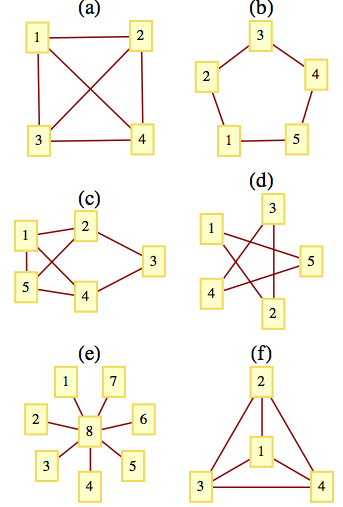
\includegraphics[width=1\linewidth]{images/fig-exercise-9-6-3.png}
\caption{What are the chromatic numbers?
                \label{fig-exercise-9-6-3}}
\end{figure}
\par\smallskip
\par\smallskip
\noindent\textbf{Answer.}\hypertarget{answer-17}{}\quad
\leavevmode%
\begin{multicols}{3}
\begin{enumerate}[label=\alph*]
\item\hypertarget{li-134}{} 3%
\item\hypertarget{li-135}{}  3%
\item\hypertarget{li-136}{}  3%
\item\hypertarget{li-137}{}  3%
\item\hypertarget{li-138}{}  2%
\item\hypertarget{li-139}{}  4%
\end{enumerate}
\end{multicols}
%
\item[4.]\hypertarget{exercise-45}{} Prove that if an undirected graph has a subgraph that is a \(K_3\) it then its chromatic number is at least 3.%
\par\smallskip
\item[5.]\hypertarget{exercise-46}{} What is \(\chi \left(K_n\right)\), \(n\geq 1\)?%
\par\smallskip
\par\smallskip
\noindent\textbf{Answer.}\hypertarget{answer-18}{}\quad
 The chromatic number is \(n\) since every vertex is connected to every other vertex.
%
\item[6.]\hypertarget{exercise-47}{} What is the chromatic number of the United States? %
\par\smallskip
\end{exercisegroup}
\par\smallskip\noindent
\hypertarget{exercisegroup-11}{}\typeout{************************************************}
\typeout{Introduction  }
\typeout{************************************************}
B Exercises%
\begin{exercisegroup}
\item[7.]\hypertarget{exercise-48}{} Complete the proof of \hyperref[theorem-euler-formula]{Theorem~\ref{theorem-euler-formula}}%
\par\smallskip
\par\smallskip
\noindent\textbf{Answer.}\hypertarget{answer-19}{}\quad
 Suppose that \(G'\) is not connected. Then \(G'\) is made up of 2 components that are planar graphs with less than \(k\) edges, \(G_1\)
and \(G_2\). For \(i=1,2\) let \(v_i,r_i, \text{and} e_i\) be the number of vertices, regions and edges in \(G_i\). By the induction hypothesis, \(v_i+r_i-e_i=2\) for \(i=1,2\)%
\par
One of the regions, the infinite one, is common to both graphs. Therefore, when we add edge \(e\) back to the graph, we have \(r=r_1+r_2-1\),
\(v=v_1+v_2\),
and  \(e=e_1+e_2+1\).

\begin{equation*}
\begin{split}
v+r-e &=\left(v_1+v_2\right)+\left(r_1+r_2-1\right)-\left(e_1+e_2+1\right)\\
	&=\left(v_1+r_1-e_1\right)+\left(v_2+r_2-e_2\right)-2\\
	&=2 + 2 -2\\
	&=2
\end{split}
\end{equation*}
%
\item[8.]\hypertarget{exercise-49}{} Use the outline of a proof of \hyperref[theorem-edge-bound]{Theorem~\ref{theorem-edge-bound}} to write a complete proof. Be sure to point out where the premise \(v\geq 3\) is essential.%
\par\smallskip
\item[9.]\hypertarget{exercise-50}{} Let \(G = (V,E)\) with \(|V|\geq 11\), and let \(U\) be the set of all undirected edges between distinct vertices in \(V\).  Prove
that either \(G\) or \(G' = \left(V,E^c\right)\) is nonplanar.%
\par\smallskip
\par\smallskip
\noindent\textbf{Answer.}\hypertarget{answer-20}{}\quad
 Since \(\left| E\right| +E^c=\frac{n(n-1)}{2}\), either \(E \text{or} E^c\) has at least \(\frac{n(n-1)}{4}\) elements. Assume that it is \textit{
E} that is larger. Since \(\frac{n(n-1)}{4}\) is greater than \(3n-6\text{  }\text{for}\text{  }n\geqslant 11\), \(G\) would be nonplanar.
Of course, if \(E^c\) is larger, then \(G'\) would be nonplanar by the same reasoning.
%
\item[10.]\hypertarget{exercise-51}{} Design an algorithm to determine whether a graph is bipartite.%
\par\smallskip
\item[11.]\hypertarget{exercise-52}{} Prove that a bipartite graph with an odd number of vertices greater than or equal to 3 has no Hamiltonian circuit.%
\par\smallskip
\par\smallskip
\noindent\textbf{Answer.}\hypertarget{answer-21}{}\quad
Suppose that \((V,E)\) is bipartite (with colors red and blue), \(\left| E\right|\) is odd, and \(\left(v_1,v_2,\ldots ,v_{2n+1},v_1\right)\)
is a Hamiltonian circuit. If \(v_1\) is red, then \(v_{2n+1}\) would also be red. But then \(\left\{v_{2n+1},v_1\right\}\) would not be in \(E\), a contradiction.
%
\end{exercisegroup}
\par\smallskip\noindent
\hypertarget{exercisegroup-12}{}\typeout{************************************************}
\typeout{Introduction  }
\typeout{************************************************}
C Exercises%
\begin{exercisegroup}
\item[12.]\hypertarget{exercise-53}{}Prove that any graph with a finite number of vertices can be drawn in three dimensions so that no edges intersect.%
\par\smallskip
\item[13.]\hypertarget{exercise-54}{}Suppose you had to color the edges of an undirected graph so that for each vertex, the edges that it is connected to have different colors.
How can this problem be transformed into a vertex coloring problem?%
\par\smallskip
\par\smallskip
\noindent\textbf{Answer.}\hypertarget{answer-22}{}\quad
 Draw a graph with one vertex for each edge, If two edges in the original graph meet at the same vertex, then draw an edge connecting the corresponding  vertices in the new graph.%
\item[14.]\hypertarget{exercise-55}{}\leavevmode%
\begin{enumerate}[label=\alph*]
\item\hypertarget{li-140}{}Suppose the edges of a \(K_6\) are colored either red or blue. Prove that there will be either a ``red \(K_3\)'' (a subset
of the vertex set with three vertices connected by red edges) or a ``blue \(K_3\)'' %
\item\hypertarget{li-141}{} Suppose six people are selected at random. Prove that either there exists a subset of three of them with the property that any two people in
the subset can communicate in a common language, or there exist three people, no two of whom can communicate in a common language.
%
\end{enumerate}
%
\par\smallskip
\end{exercisegroup}
\par\smallskip\noindent
%
\backmatter
%
%
%% A lineskip in table of contents as transition to appendices, backmatter
\addtocontents{toc}{\vspace{\normalbaselineskip}}
%
\typeout{************************************************}
\typeout{References  References}
\typeout{************************************************}
\chapter[References]{References}\label{references-1}
%% If this is a top-level references
%%   you can replace with "thebibliography" environment
\begin{referencelist}
\bibitem[1]{biblio-sopowit-1983}\hypertarget{biblio-sopowit-1983}{}Sopowit, K. J., E. M. Reingold, and D. A. Plaisted \textit{The Traveling Salesman Problem and Minimum Matching in the Unit Square}.SIAM J. Computing, 1983,\textbf{12}, 144\textendash{}56.
\end{referencelist}
%
%% The index is here, setup is all in preamble
\printindex
%
\end{document}